\documentclass{beamer}
\usetheme{Madrid}
\usecolortheme{default}
\usepackage[style=ieee,backend=biber]{biblatex}
\usepackage{graphicx}
\usepackage[font=scriptsize,labelfont=bf]{caption}
\addbibresource{references.bib}

\graphicspath{{img/}}

\title{Research Stay: Predictive Maintenance of Industrial Equipment}
\author{Juan Echeagaray}
\institute{Tec de Monterrey}
\date{\today}

\begin{document}
    \frame{\titlepage}

    \begin{frame}
        \frametitle{Agenda}
        \tableofcontents
    \end{frame}

    \section{Introduction}

        \begin{frame}
            \frametitle{Introduction}
            \begin{columns}
                \begin{column}{0.5\textwidth}
                    Maintenance scheduled by data analytics on historical data
                    \begin{itemize}
                        \item Enhance operational efficiency
                        \item Sustainability and cost reduction
                        \item Competitive advantage
                        \item \textbf{Safety at the forefront}
                    \end{itemize}
                \end{column}
                \begin{column}{0.5\textwidth}
                    \begin{figure}[!htbp]
                        \centering
                        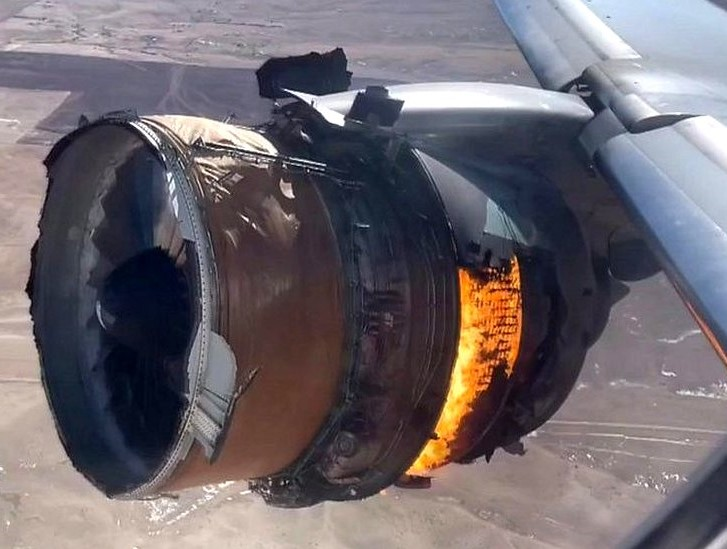
\includegraphics[scale=0.3]{turbine_failure.jpg}
                        \caption{Turbine failure mid-flight \cite{bbc-news-2021}}
                    \end{figure}
                \end{column}
            \end{columns}
        \end{frame}

    \section{Problem Statement}

        \begin{frame}
            \frametitle{Problem Statement}

            Predictive maintenance faces 2 main challenges:
            \begin{block}{Implementation}
                Need a model to estimate the RUL of a set of machinery, in an efficient and reliable manner
            \end{block}

            \begin{alertblock}{Interpretability}
                Need to \textit{understand} why a model produces a given RUL estimate, becomes more important in critical environments
            \end{alertblock}

        \end{frame}

    \section{Objectives}

        \begin{frame}
            \frametitle{Objectives}
            This research project aims to develop:
            \begin{itemize}
                \item PdM framework to predict RUL for a designated fleet of machinery
                \item Model which ensures reproducibility, stability, robustness and confidence Modelo estable, robusto, reproducible y confiable
                \item Tools to interpret and visualize the model's predictions
            \end{itemize}
        \end{frame}

    \section{Scope}

        \begin{frame}
            \frametitle{Scope}
            The previous objectives are to be accomplished subject to the following constraints and assumptions:
            \begin{itemize}
                \item RUL prediction of an uniform fleet of machines
                \item Availability of a labeled dataset with run to failure sequences of each machine
            \end{itemize}
        \end{frame}

    \section{Hypothesis}

        \begin{frame}
            \frametitle{Hypothesis}
            Throughout this research stay it is postulated:
            \begin{exampleblock}{Hypothesis}
                Using a set of sensor readings from a uniform fleet of machines in conjunction with environmental descriptors, it is possible to train an integrated predictive model for the Remaining Useful Life of an equipment, which is stable, robust, reproducible and reliable
            \end{exampleblock}
        \end{frame}

    \section{Exploratory Data Analysis}

        \begin{frame}{Exploratory Data Analysis}{NCMAPSS Dataset}

            Flight conditions and readings from a fleet of turbofan engines,
            derived from NASA's CMAPSS model, including real flight conditions and relates the degradation process to the operating history of the machine. \cite{arias2021aircraft}
            \begin{itemize}
                \item Used in the PHMAP 2021 Data Challenge \cite{phm-conference}
                \item State of the art prognosis dataset (akin to MNIST and CIFAR for CV)
            \end{itemize}

            \begin{figure}[!htbp]
                \centering
                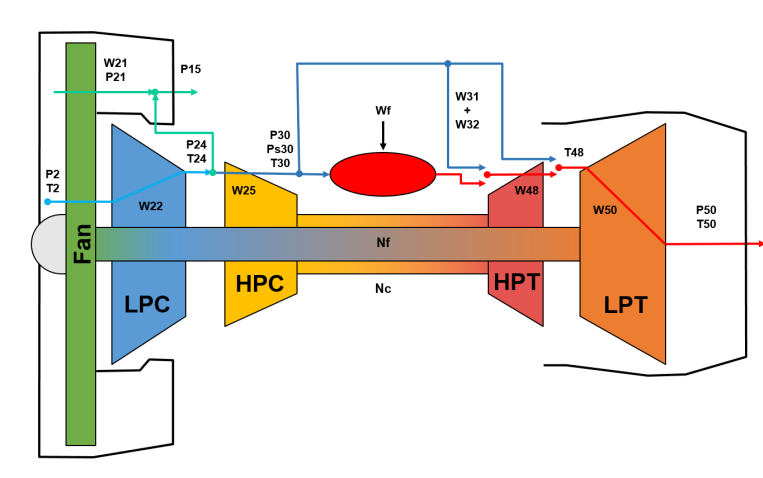
\includegraphics[scale=0.35]{cmapss_turbofan.png}
                \caption{CMAPSS turbofan engine schematic}
            \end{figure}
        \end{frame}

        \begin{frame}{Exploratory Data Analysis}{Data Overview}
            \begin{columns}
                \begin{column}{0.4\textwidth}
                    \begin{itemize}
                        \item Split into 10 h5 files
                        \item Sampling frequency of 1 second
                        \item Contains sensor readings, environmental descriptors, auxiliary variables, virtual sensor readings and RUL values
                        \item Corrupted file in the dataset
                    \end{itemize}
                \end{column}
                \begin{column}{0.6\textwidth}
                    \begin{table}[!htbp]
                        \centering
                        \scalebox{0.5}{
                        \begin{tabular}{ |l|l|l| }
                            \hline
                            Symbol & Description & Units \\
                            \hline
                            alt & Altitude & ft \\
                            Mach & Flight Mach number & - \\
                            TRA & Throttle-resolver angle & \% \\
                            T2 & Total temperature at fan inlet & °R \\
                            \hline
                            Wf & Fuel flow & pps \\
                            Nf & Physical fan speed & rpm \\
                            Nc & Physical core speed & rpm \\
                            T24 & Total temperature at LPC outlet & °R \\
                            T30 & Total temperature at HPC outlet & °R \\
                            T48 & Total temperature at HPT outlet & °R \\
                            T50 & Total temperature at LPT outlet & °R \\
                            P15 & Total pressure in bypass-duct & psia \\
                            P2 & Total pressure at fan inlet & psia \\
                            P21 & Total pressure at fan outlet & psia \\
                            P24 & Total pressure at LPC outlet & psia \\
                            Ps30 & Static pressure at HPC outlet & psia \\
                            P40 & Total pressure at burner outlet & psia \\
                            P50 & Total pressure at LPT outlet & psia \\
                            \hline
                            RUL & Remaining Useful Life & cycles \\
                            \hline
                            unit & Unit number & - \\
                            cycle & Flight cycle number & - \\
                            Fc & Flight class & - \\
                            hs & Health state & - \\
                            \hline
                        \end{tabular}}
                        \label{tab:dataset_info}
                        \caption{General description of dataset variables  \cite{phm-conference}}
                    \end{table}
                \end{column}
            \end{columns}

        \end{frame}

        \begin{frame}{Exploratory Data Analysis}{Flight Class Distribution}
            \begin{figure}[!htbp]
                \centering
                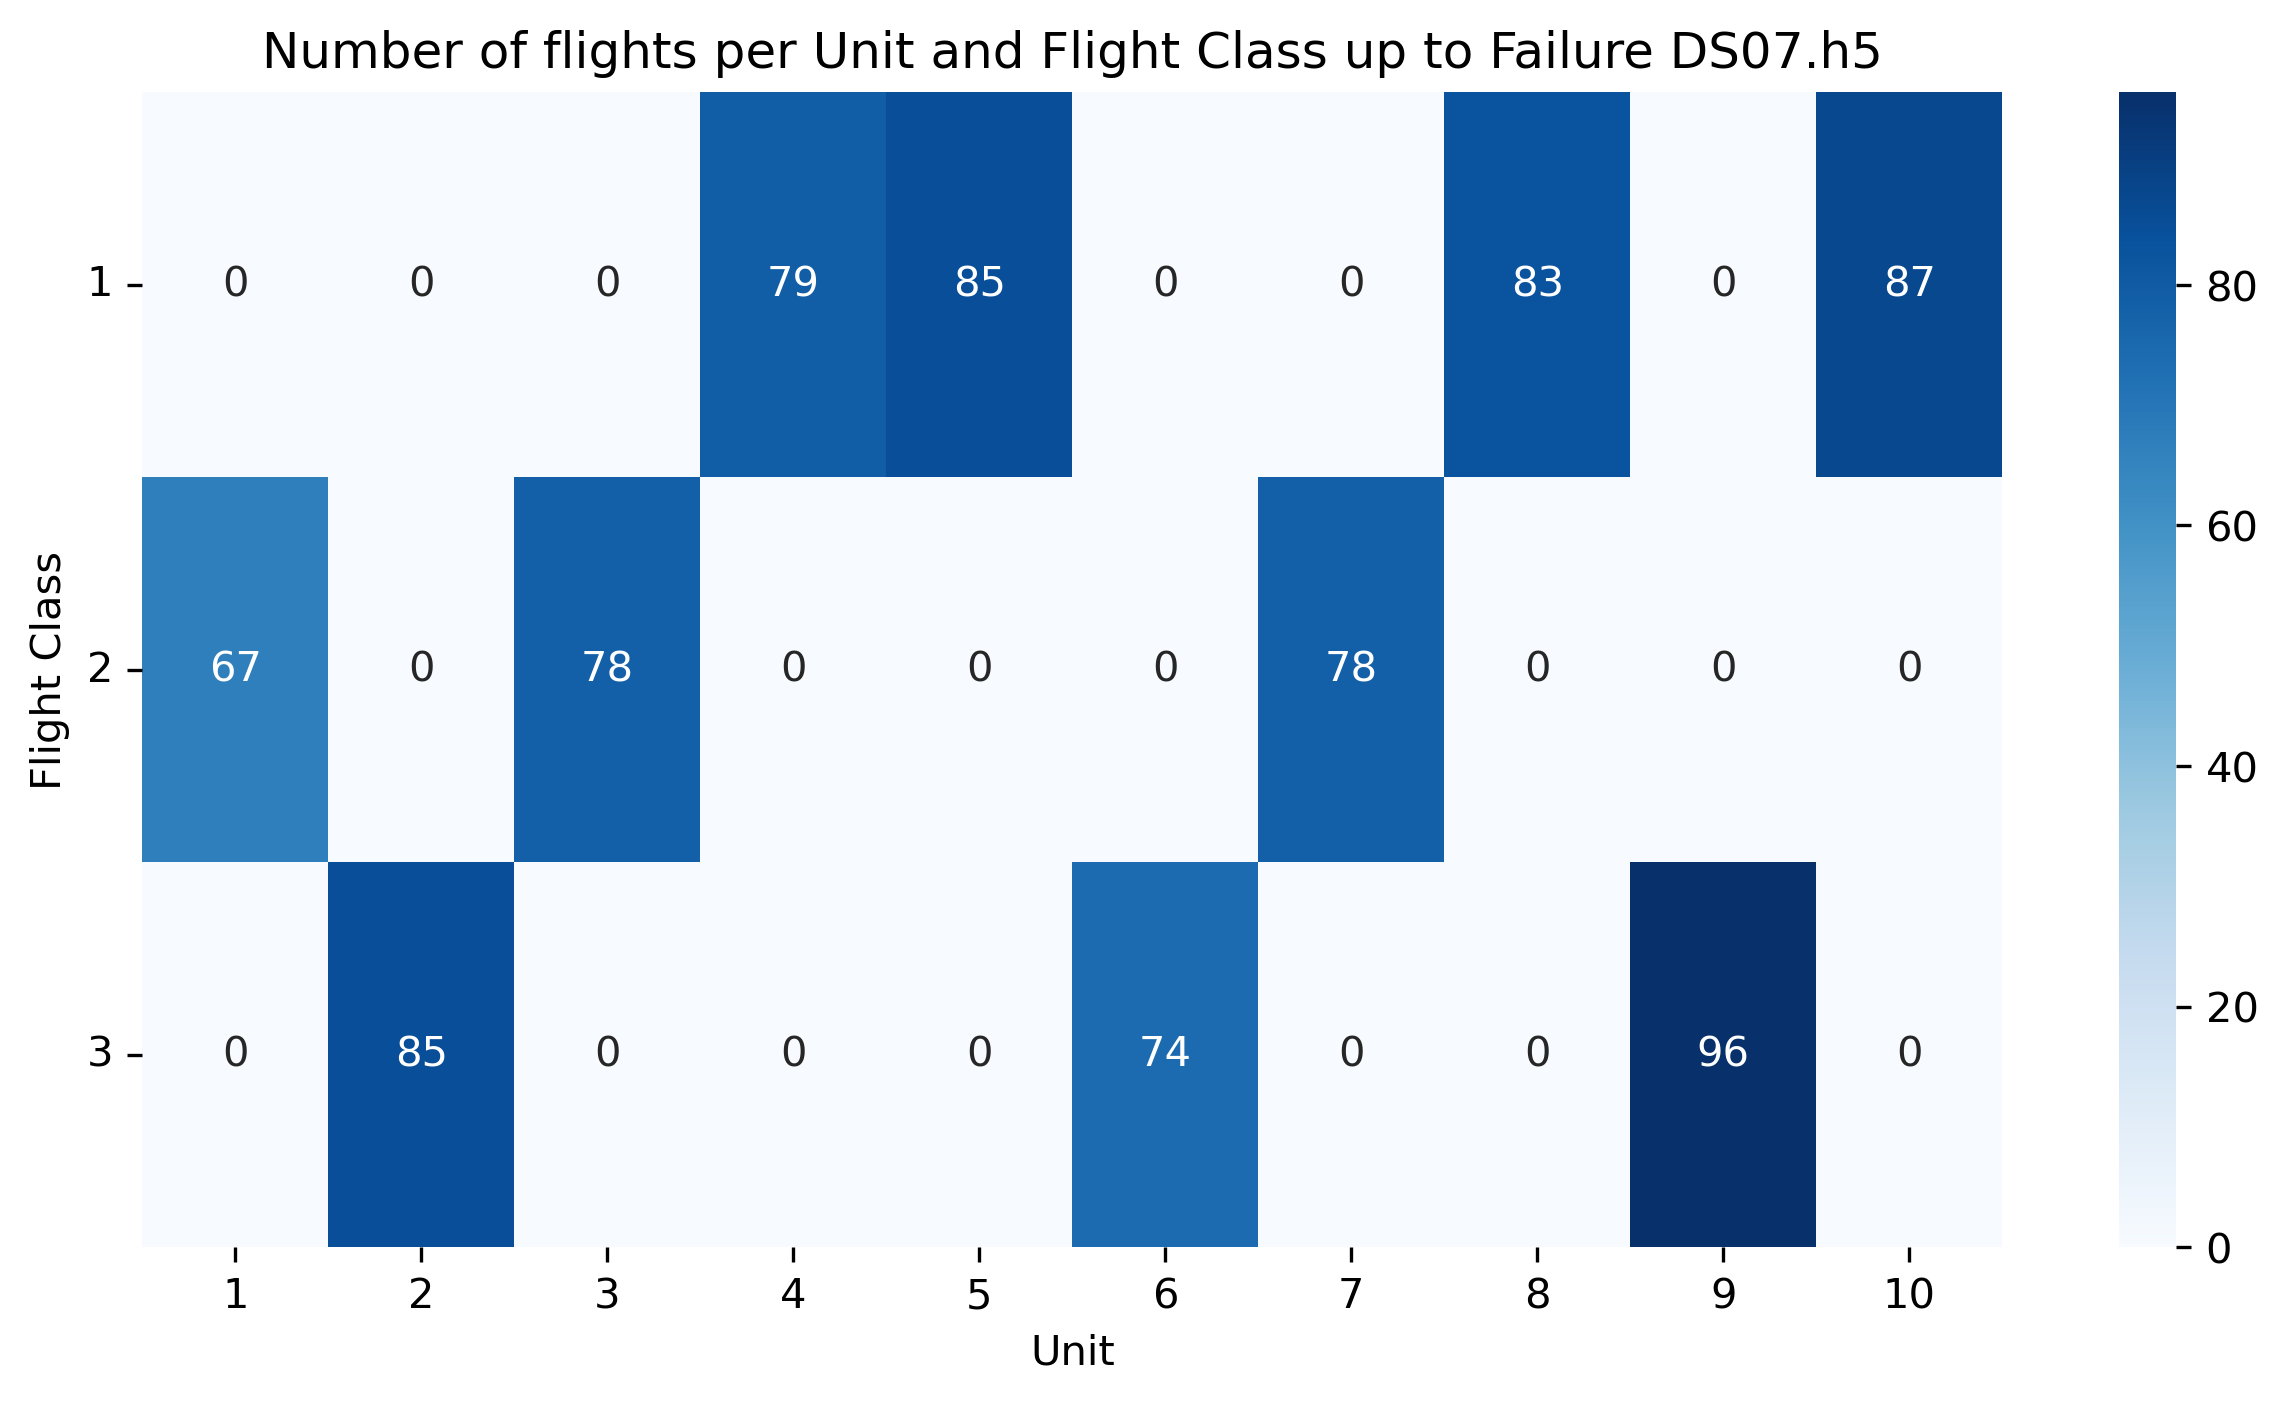
\includegraphics[scale=0.4]{fligt_class_per_unit_DS07.h5.png}
                \caption{Flights recorded for each class per unit}
            \end{figure}
            Flight classes encode flight duration\footnotemark[1], and there are no inter-class units
            \footnotetext[1]{FC1 ranges between 1 and 3 hours, FC2 between 3 and 5, and FC3 is greater than 5}
        \end{frame}

        \begin{frame}{Exploratory Data Analysis}{Sample Operating Conditions}
            \begin{figure}[!htbp]
                \centering
                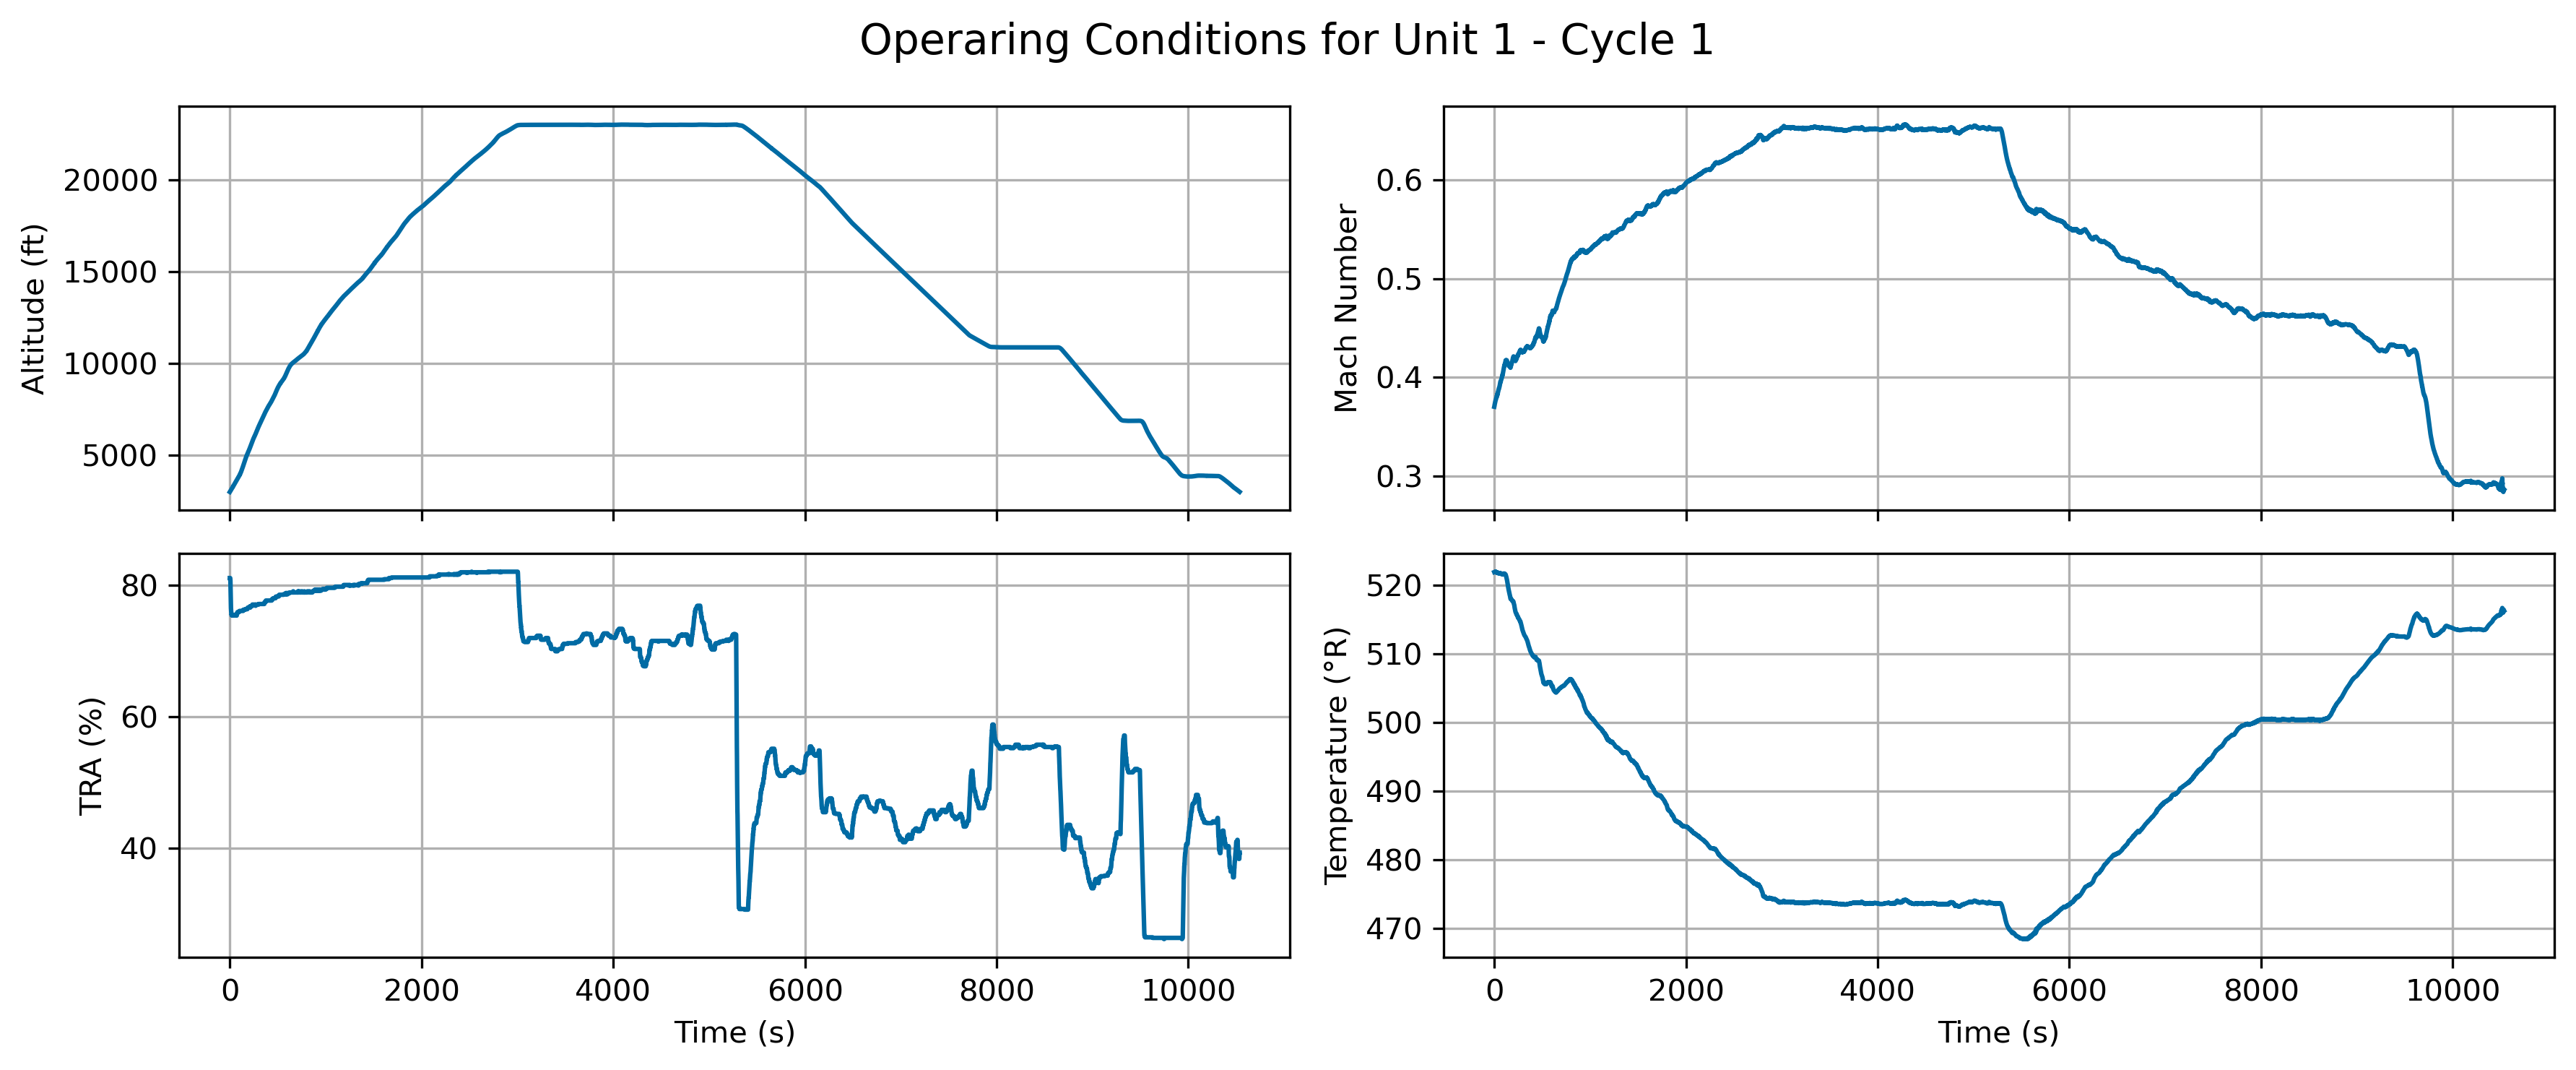
\includegraphics[scale=0.35]{operating_conditions_unit_1_cycle_1.png}
                \caption{Operating conditions for the first flight of Unit 1}
            \end{figure}
        \end{frame}

        \begin{frame}{Exploratory Data Analysis}{Sample Operating Conditions}
            \begin{figure}[!htbp]
                \centering
                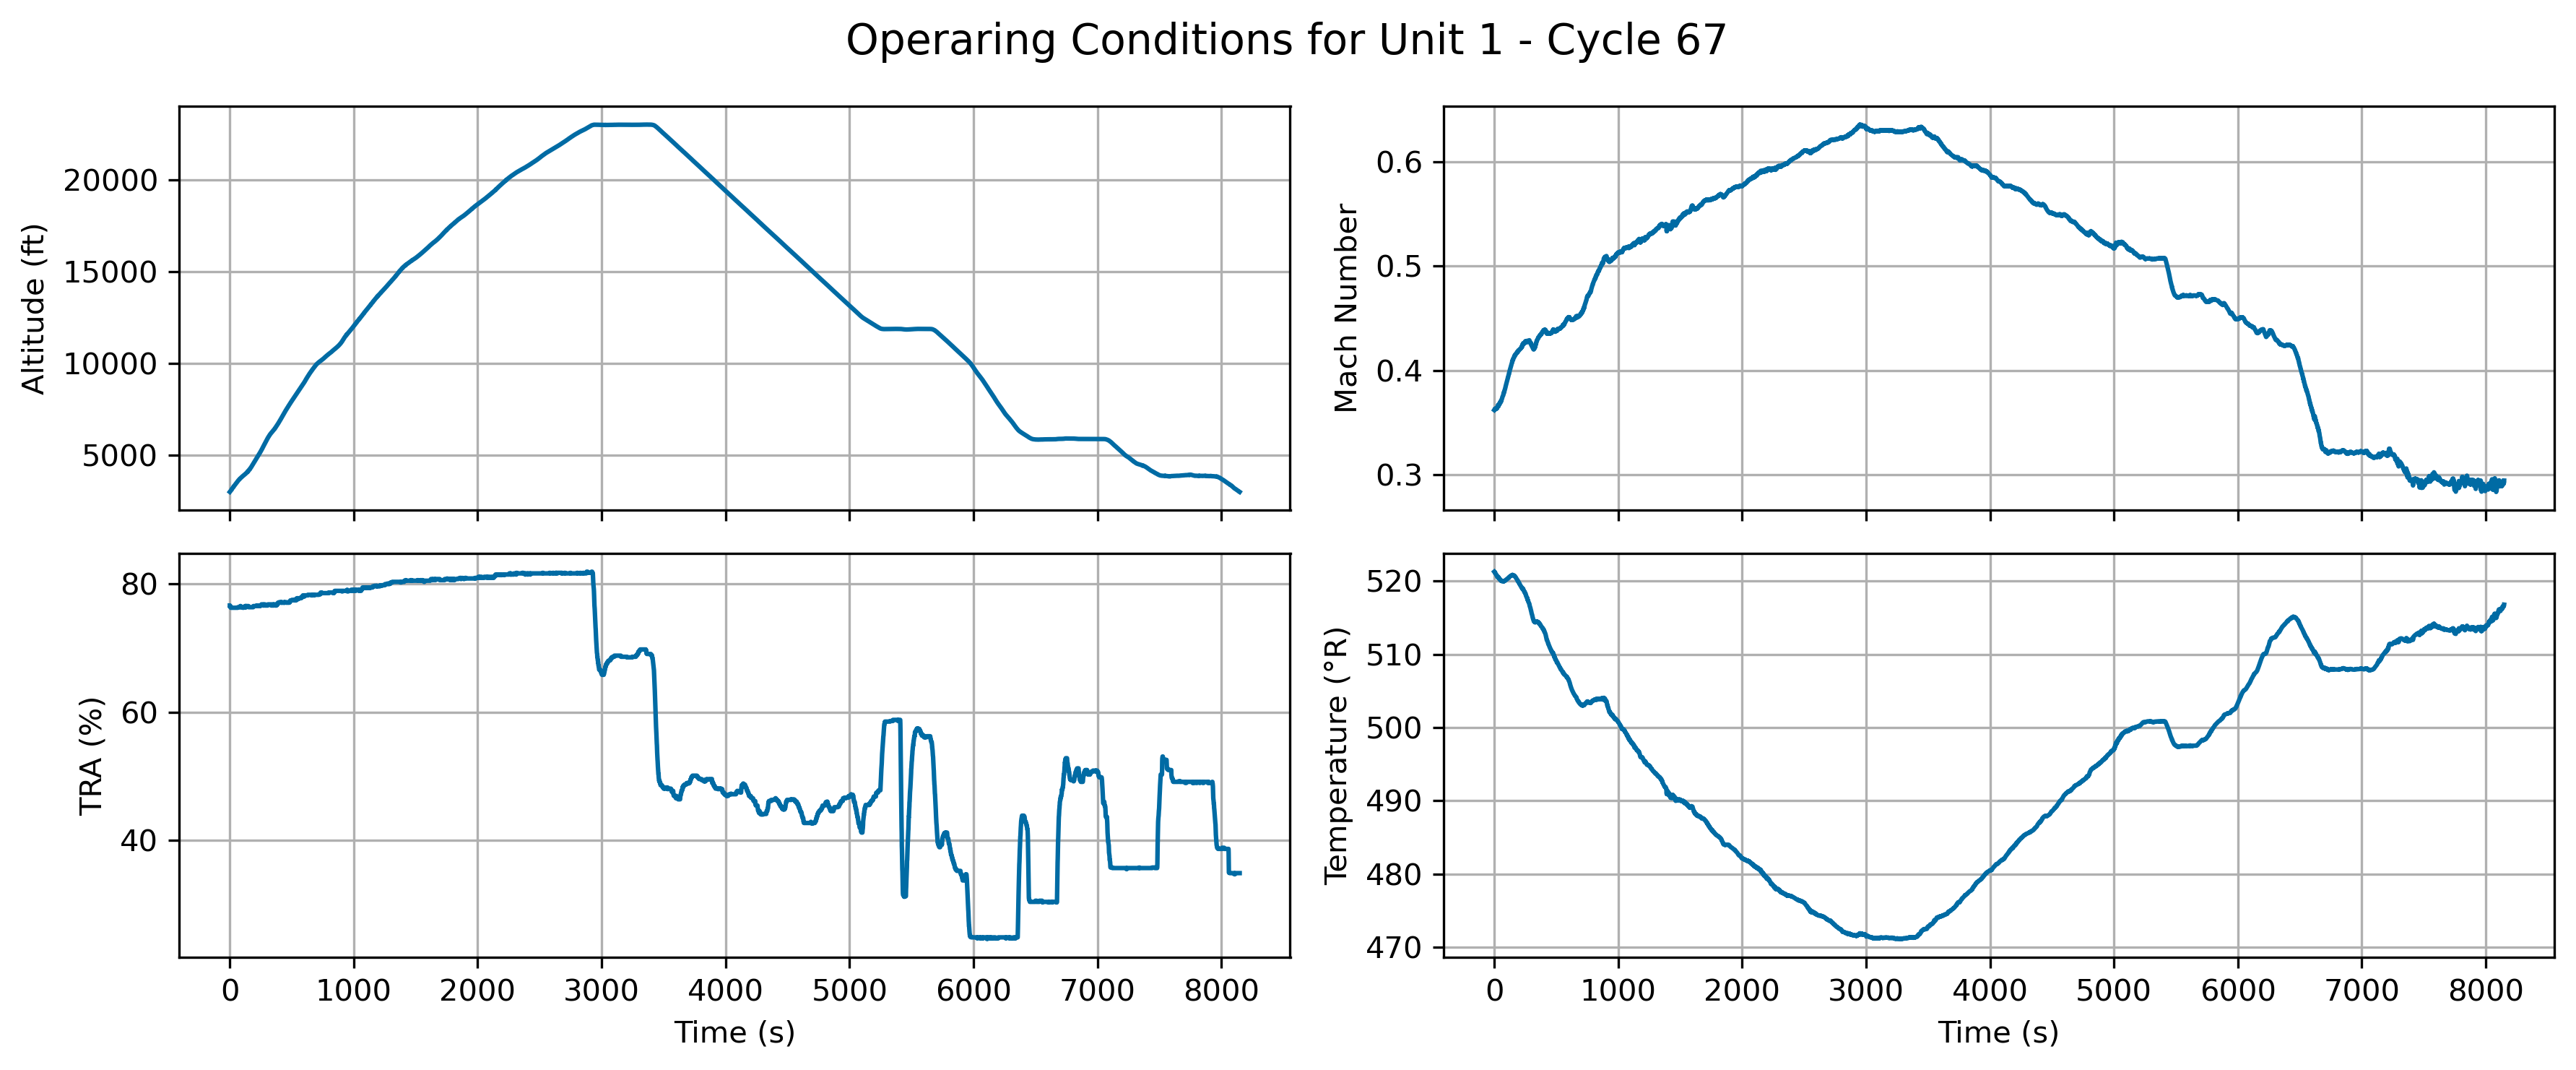
\includegraphics[scale=0.35]{operating_conditions_unit_1_cycle_67.png}
                \caption{Operating conditions for the last flight of Unit 1 (EOL)}
            \end{figure}
        \end{frame}

        \begin{frame}{Exploratory Data Analysis}{Operating Conditions per Flight Class}
            \begin{figure}[!htbp]
                \centering
                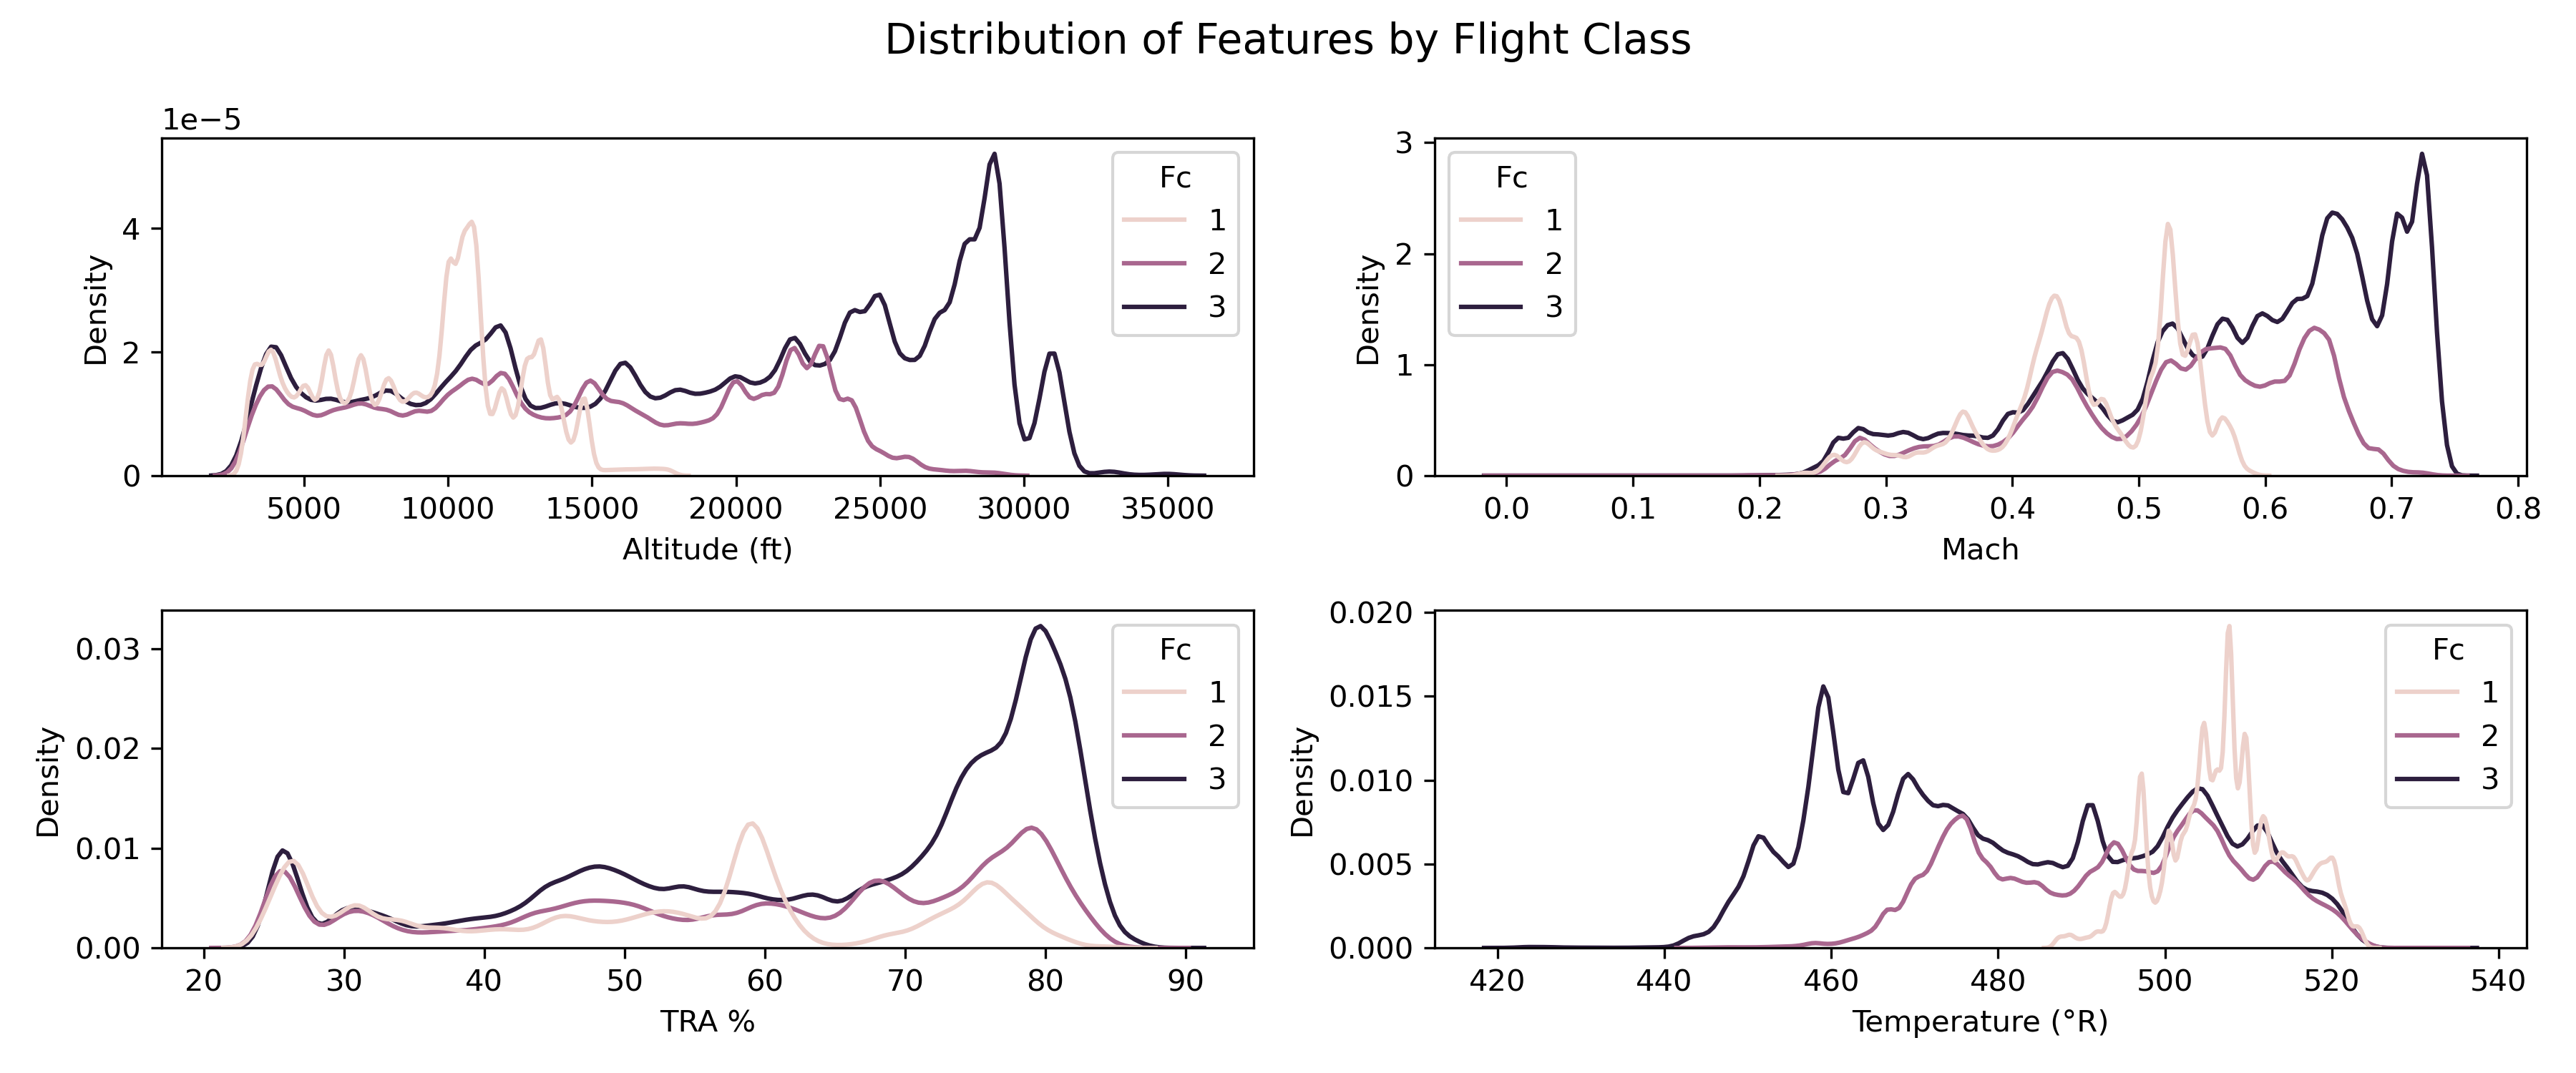
\includegraphics[scale=0.35]{features_per_condition_fc.png}
                \caption{Distribution of operating conditions per Flight Class}
            \end{figure}

            Distinctive operating conditions per FC where FC2 can be seen as a mixture of FC1 and FC3
        \end{frame}

        \begin{frame}{Exploratory Data Analysis}{Altitude and Mach Number}
            \begin{figure}[!htbp]
                \centering
                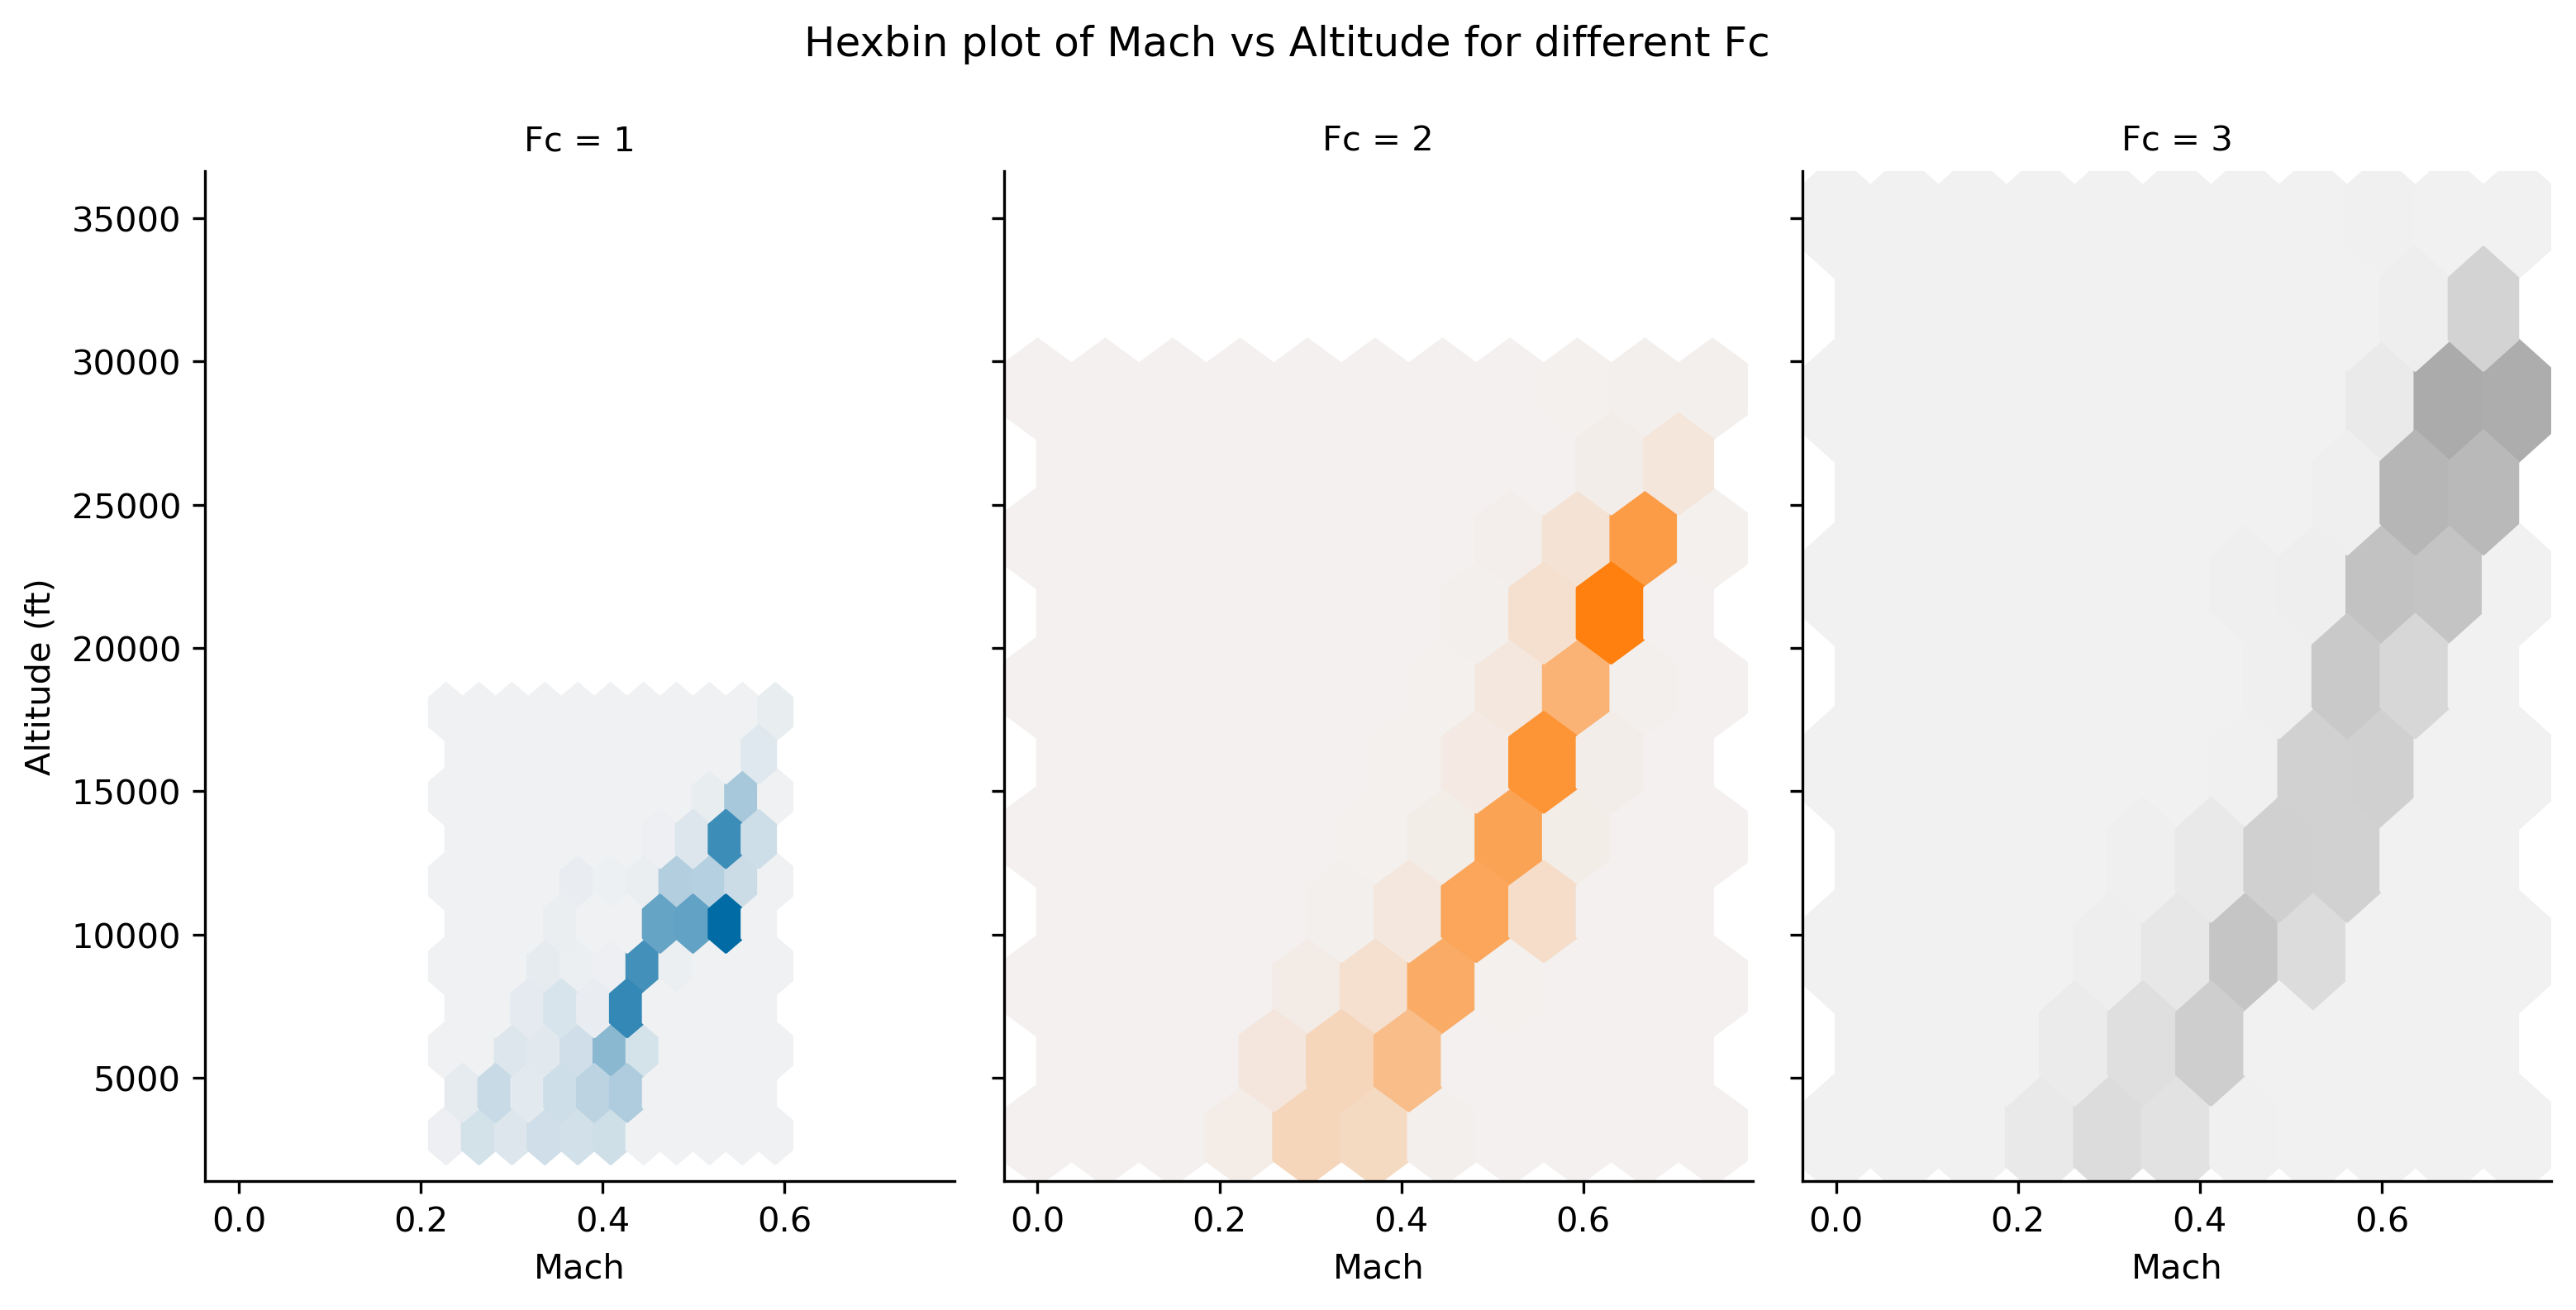
\includegraphics[scale=0.35]{mach_altitude.png}
                \caption{General relationship between Altitude and Mach Number}
            \end{figure}

            General alignment in FC2 and FC3, but FC1 has a higher dispersion \footnote{Potentially caused by the shorter flight duration}
        \end{frame}

        \begin{frame}{Exploratory Data Analysis}{Initial Sensor Readings}
            \begin{figure}[!htbp]
                \centering
                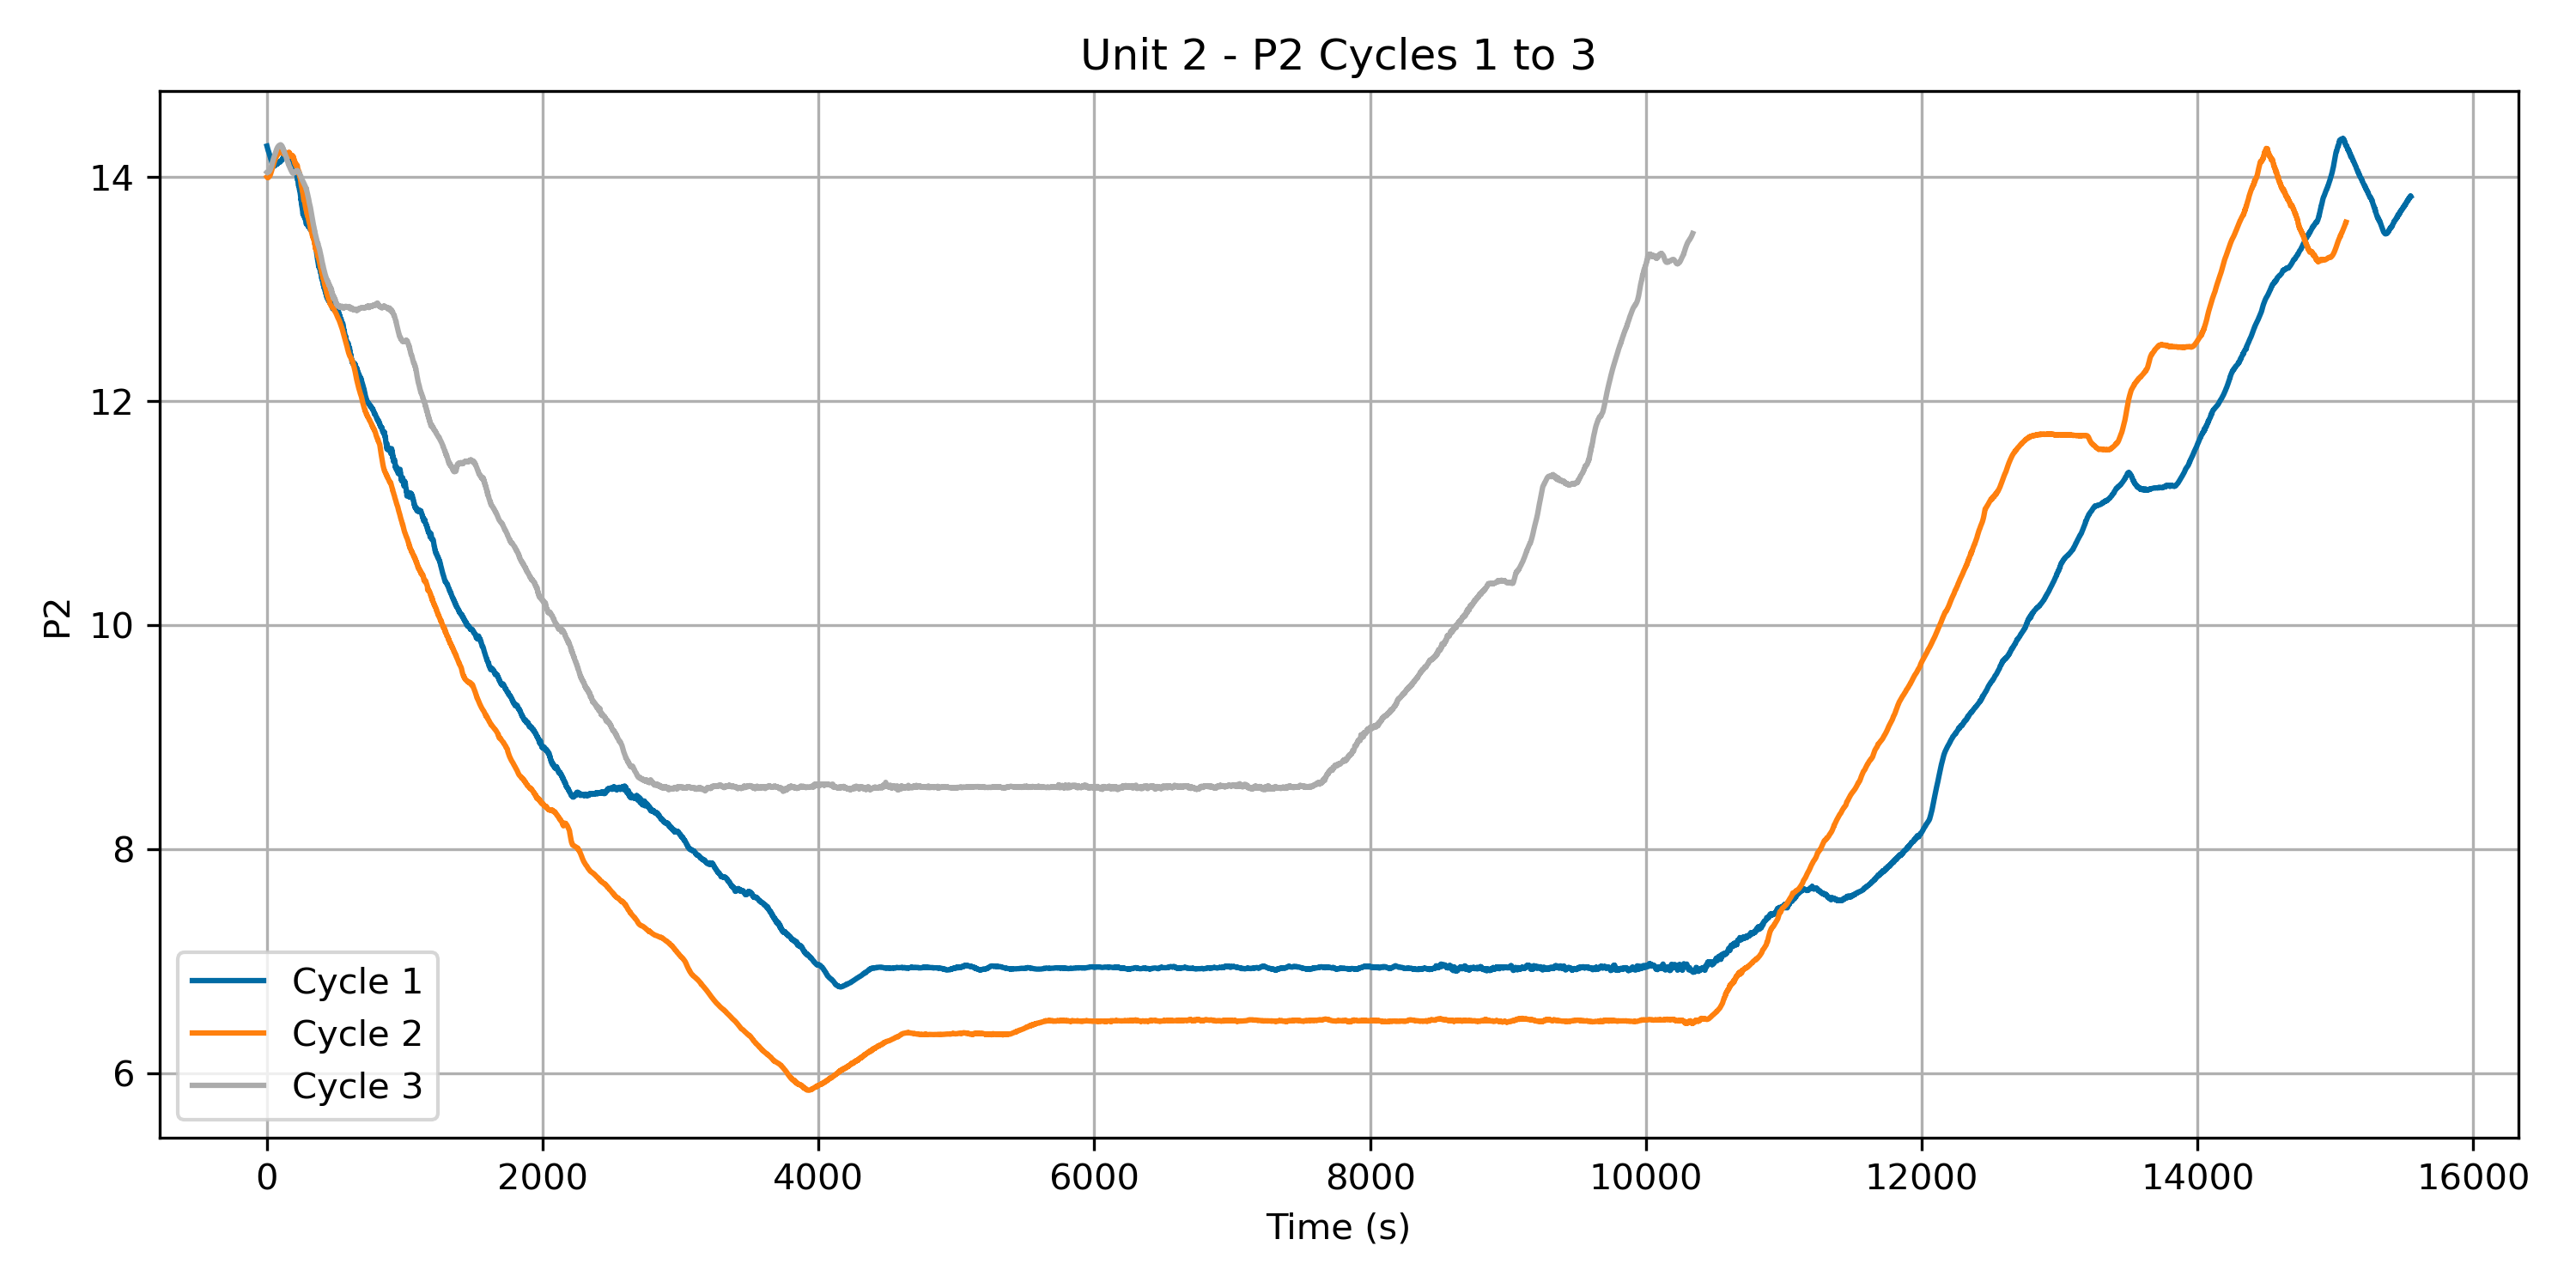
\includegraphics[scale=0.35]{unit_2_P2_cycles_1_3.png}
                \caption{Total Pressure at fan inlet (P2) for the first 3 cycles of unit 2}
            \end{figure}
            Mostly smooth readings with predictable abrupt changes
        \end{frame}

        \begin{frame}{Exploratory Data Analysis}{Final Sensor Readings}
            \begin{figure}[!htbp]
                \centering
                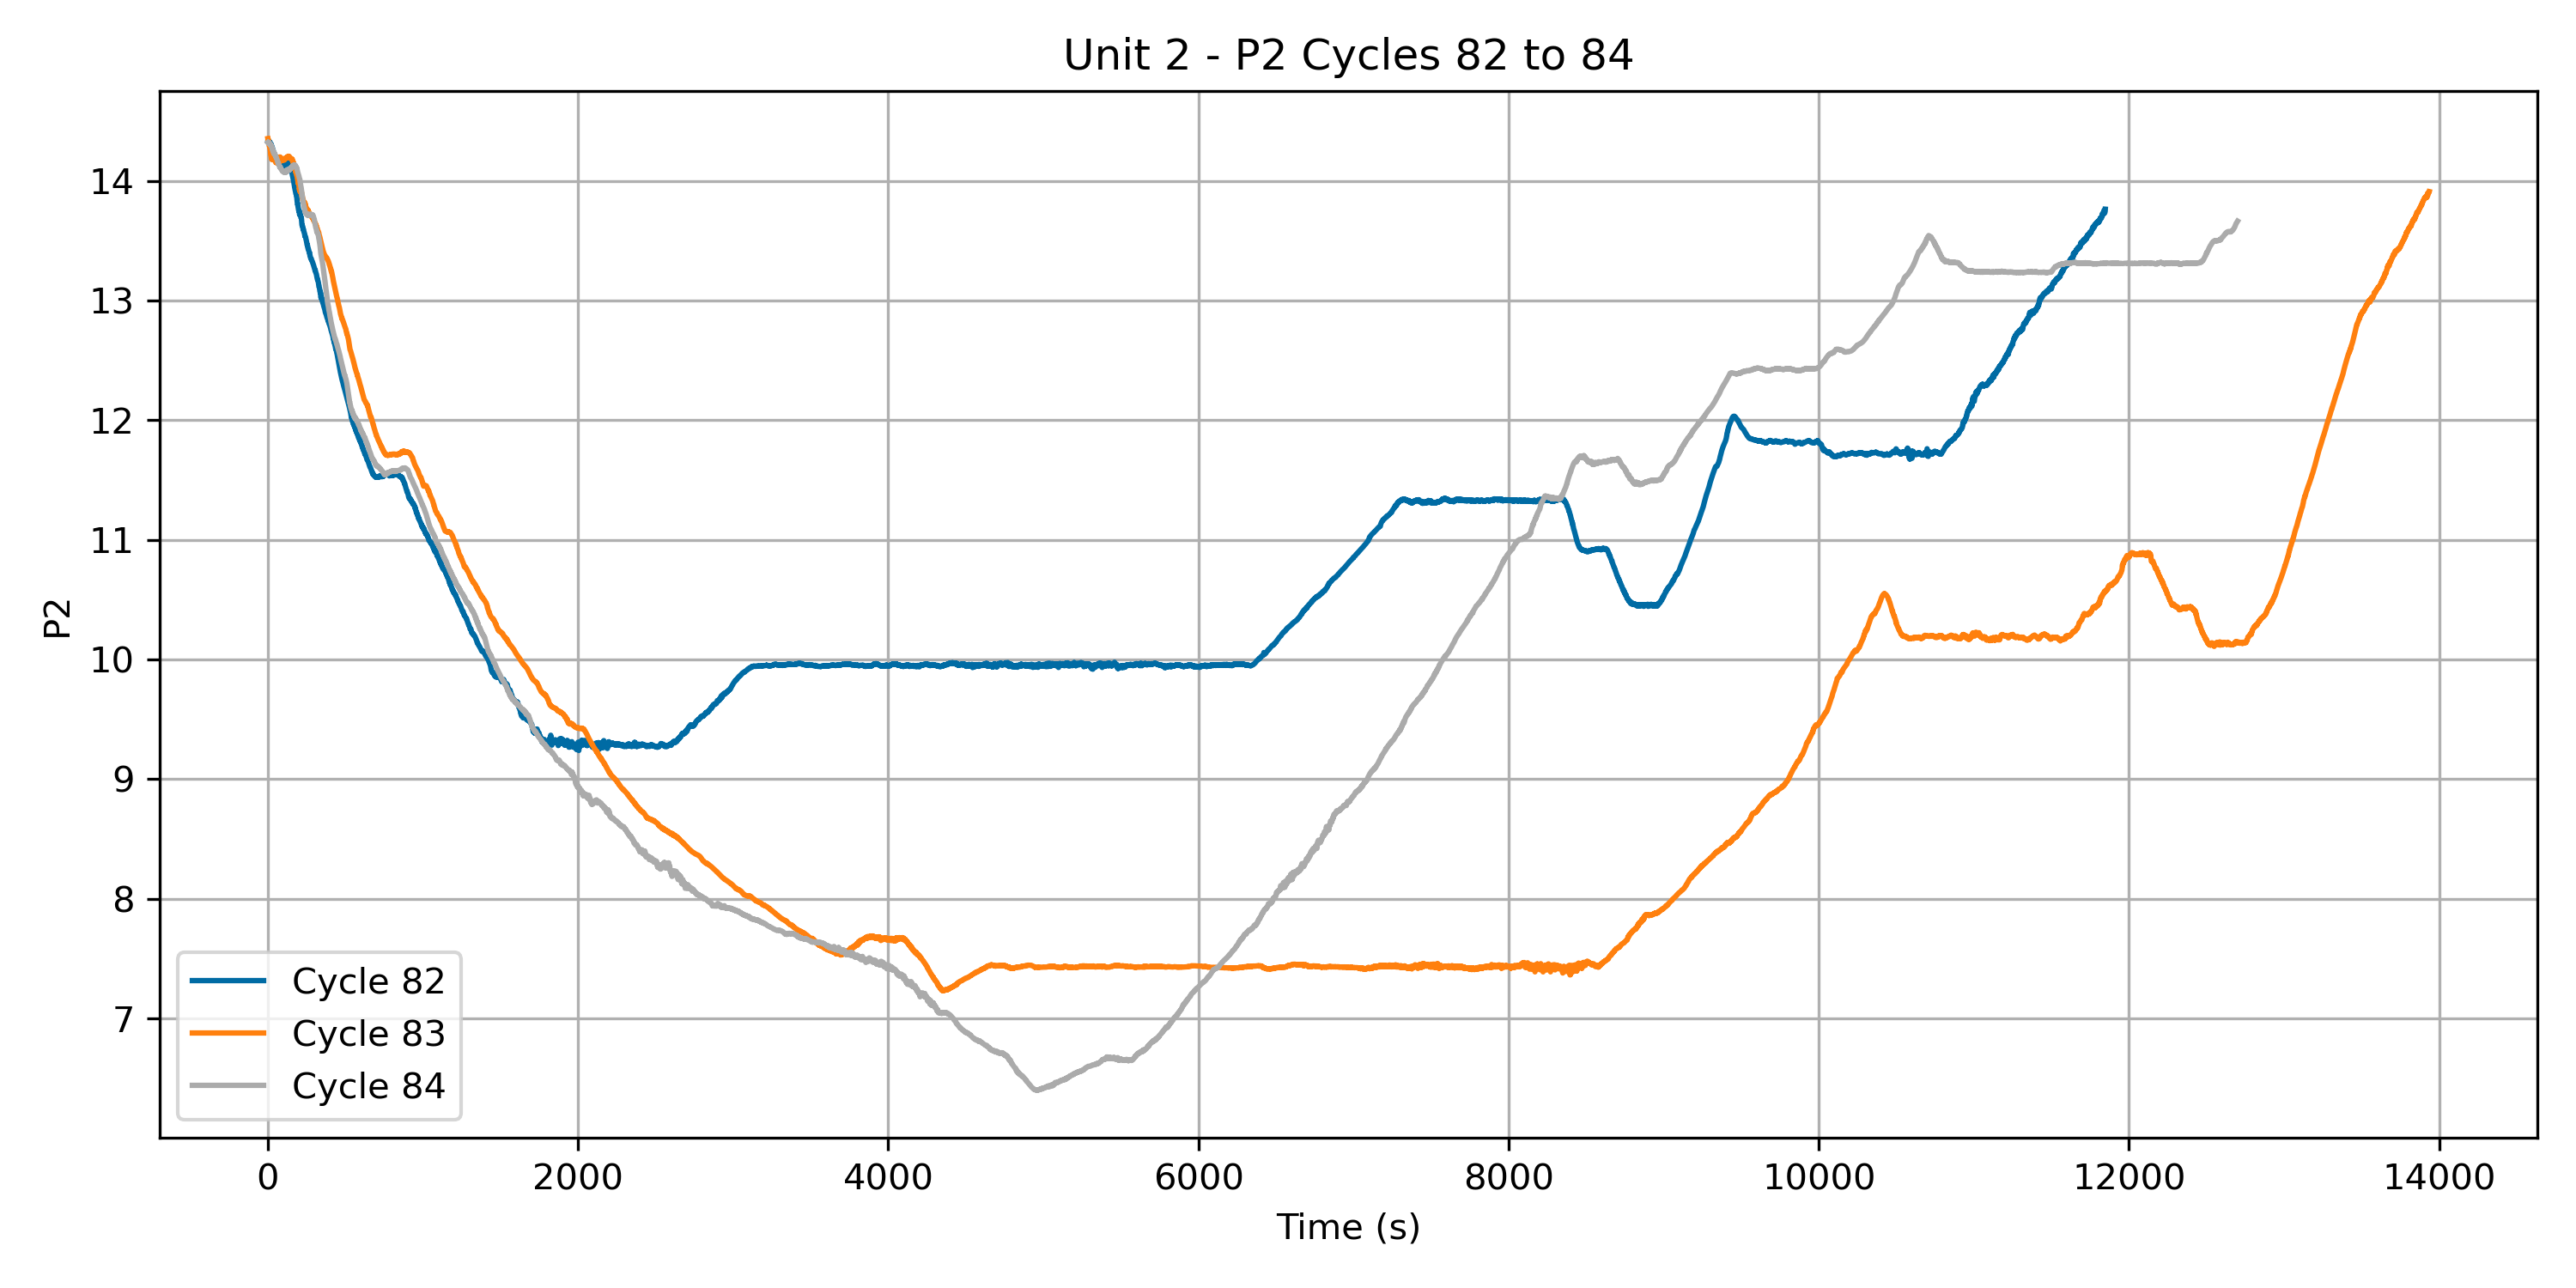
\includegraphics[scale=0.35]{unit_2_P2_cycles_82_84.png}
                \caption{Total Pressure at fan inlet (P2) for the last 3 cycles of unit 2}
            \end{figure}
            Smoothness degradation with a presence of new plateaus near the end of the flight
        \end{frame}

    \section{Methodology}

        \begin{frame}{Methodology}{Proposed Methodology}
            In general the framework can be broken down to:
            \begin{figure}[!htbp]
                \centering
                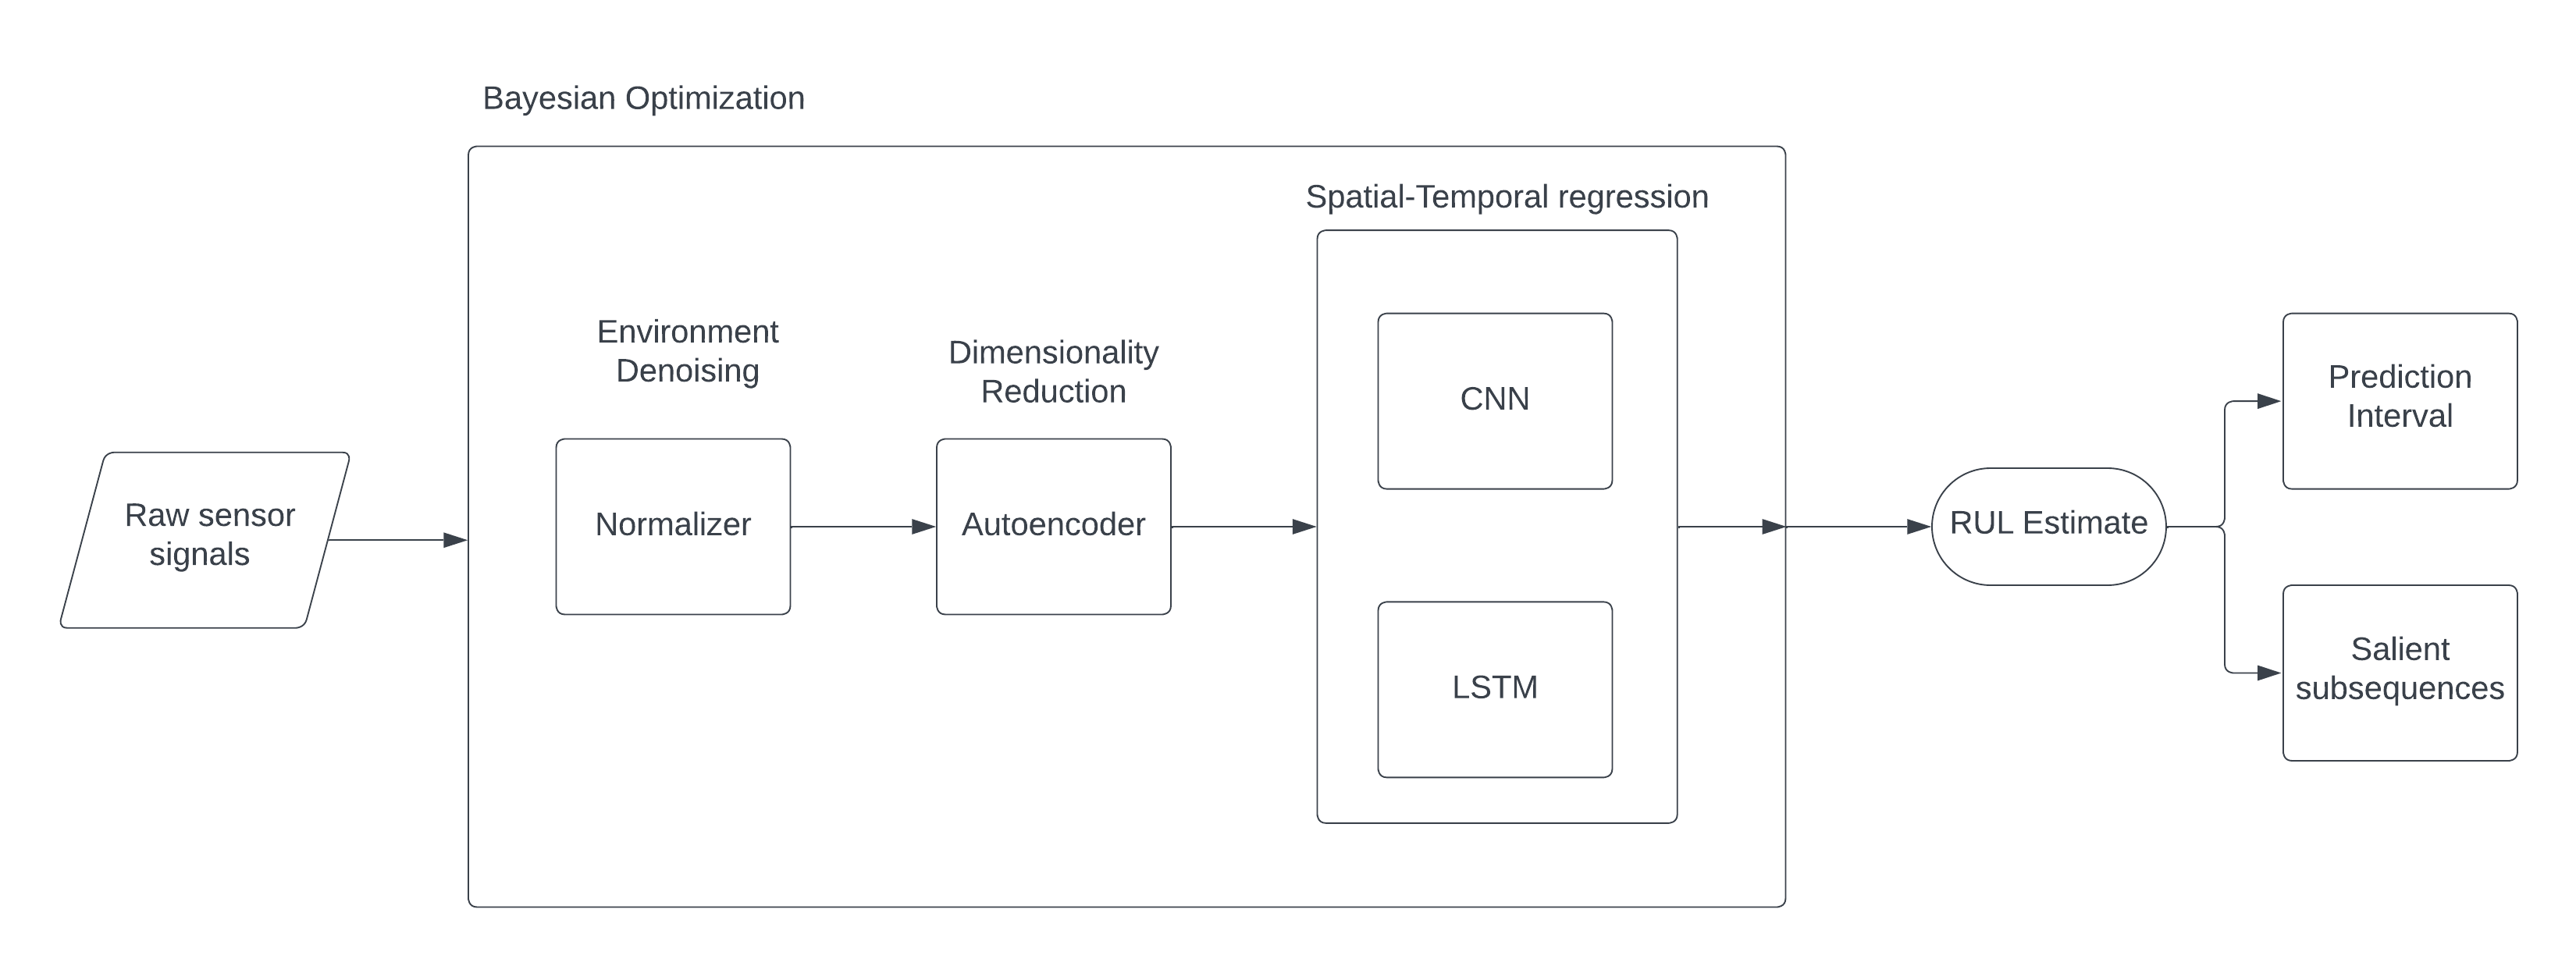
\includegraphics[scale=0.45]{pdm-ml-process.png}
                \caption{Proposed Methodology}
            \end{figure}
        \end{frame}

        \subsection{Normalizer}

            \begin{frame}
                \frametitle{Normalizer}
                RUL prediction is usually based on sensor readings of each operating cycle, but:
                \begin{itemize}
                    \item Sensor readings encoding degradation can be obfuscated by environmental conditions.
                    \item No easy way to analyze a machine's degradation without a detailed analysis
                \end{itemize}
                \begin{block}{Proposition}
                    Design a normalizer function to model a machine's degradation based upon environmental descriptors and analyzed in sensor readings
                \end{block}
            \end{frame}

            \begin{frame}
                \frametitle{Degradation Model Proposition}
                Given a vector $E_t$ of $m$ environmental descriptors and a vector $S_t$ of $n$ sensor reading variables for each timestamp $t$, a function $f$ is proposed as follows:
                \begin{equation}
                    f: \mathbb{R}^m \rightarrow \mathbb{R}^n
                \end{equation}

                The function $f$ is then an internal model of how $S_t$ \textbf{should} look like if the machine were healthy.

                The normalized measures for each timestamp will be:
                \begin{equation}
                    \hat{S}_t = S_t - f(E_t)
                \end{equation}
            \end{frame}

            \begin{frame}
                \frametitle{Degradation Model Learning}
                Prepare a subset of data where the machine is known to operate in optimal conditions and use a neural network to learn the mapping $f$, the baseline architecture is then a DNN:
                \begin{figure}[!htbp]
                    \centering
                    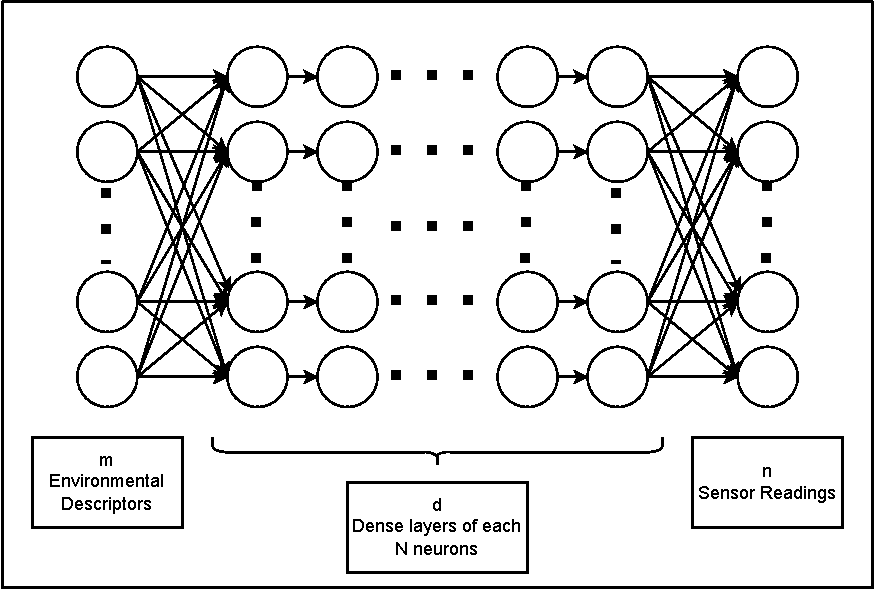
\includegraphics[scale=0.45]{descriptor_predictor_diagram.pdf}
                    \caption{Baseline sequential model for the degradation function}
                \end{figure}
            \end{frame}

    \section{Experimental Results}

        \begin{frame}{Normalizer}{Model Parameters}
            \begin{itemize}
                \item Test Dataset: NCMAPSS DS01, all FC, only failures in Low Pressure Turbine
                \item Input: Environmental descriptors, operating cycle, flight class, and time (scaled between 0 and 1)
                \item Output: Sensor readings
                \item 5 dense layers of 32 neurons each with a L2 kernel regularizer ($\lambda = 0.005$)
                \item Adamax for faster and more stable convergence rates
                \item Training for maximum number epochs of a 100 epochs with early stopping of 5\% of the maximum epochs if there's no improvement in validation loss
            \end{itemize}
        \end{frame}

        \begin{frame}{Normalizer}{Training Overview}
            \begin{figure}[!htbp]
                \centering
                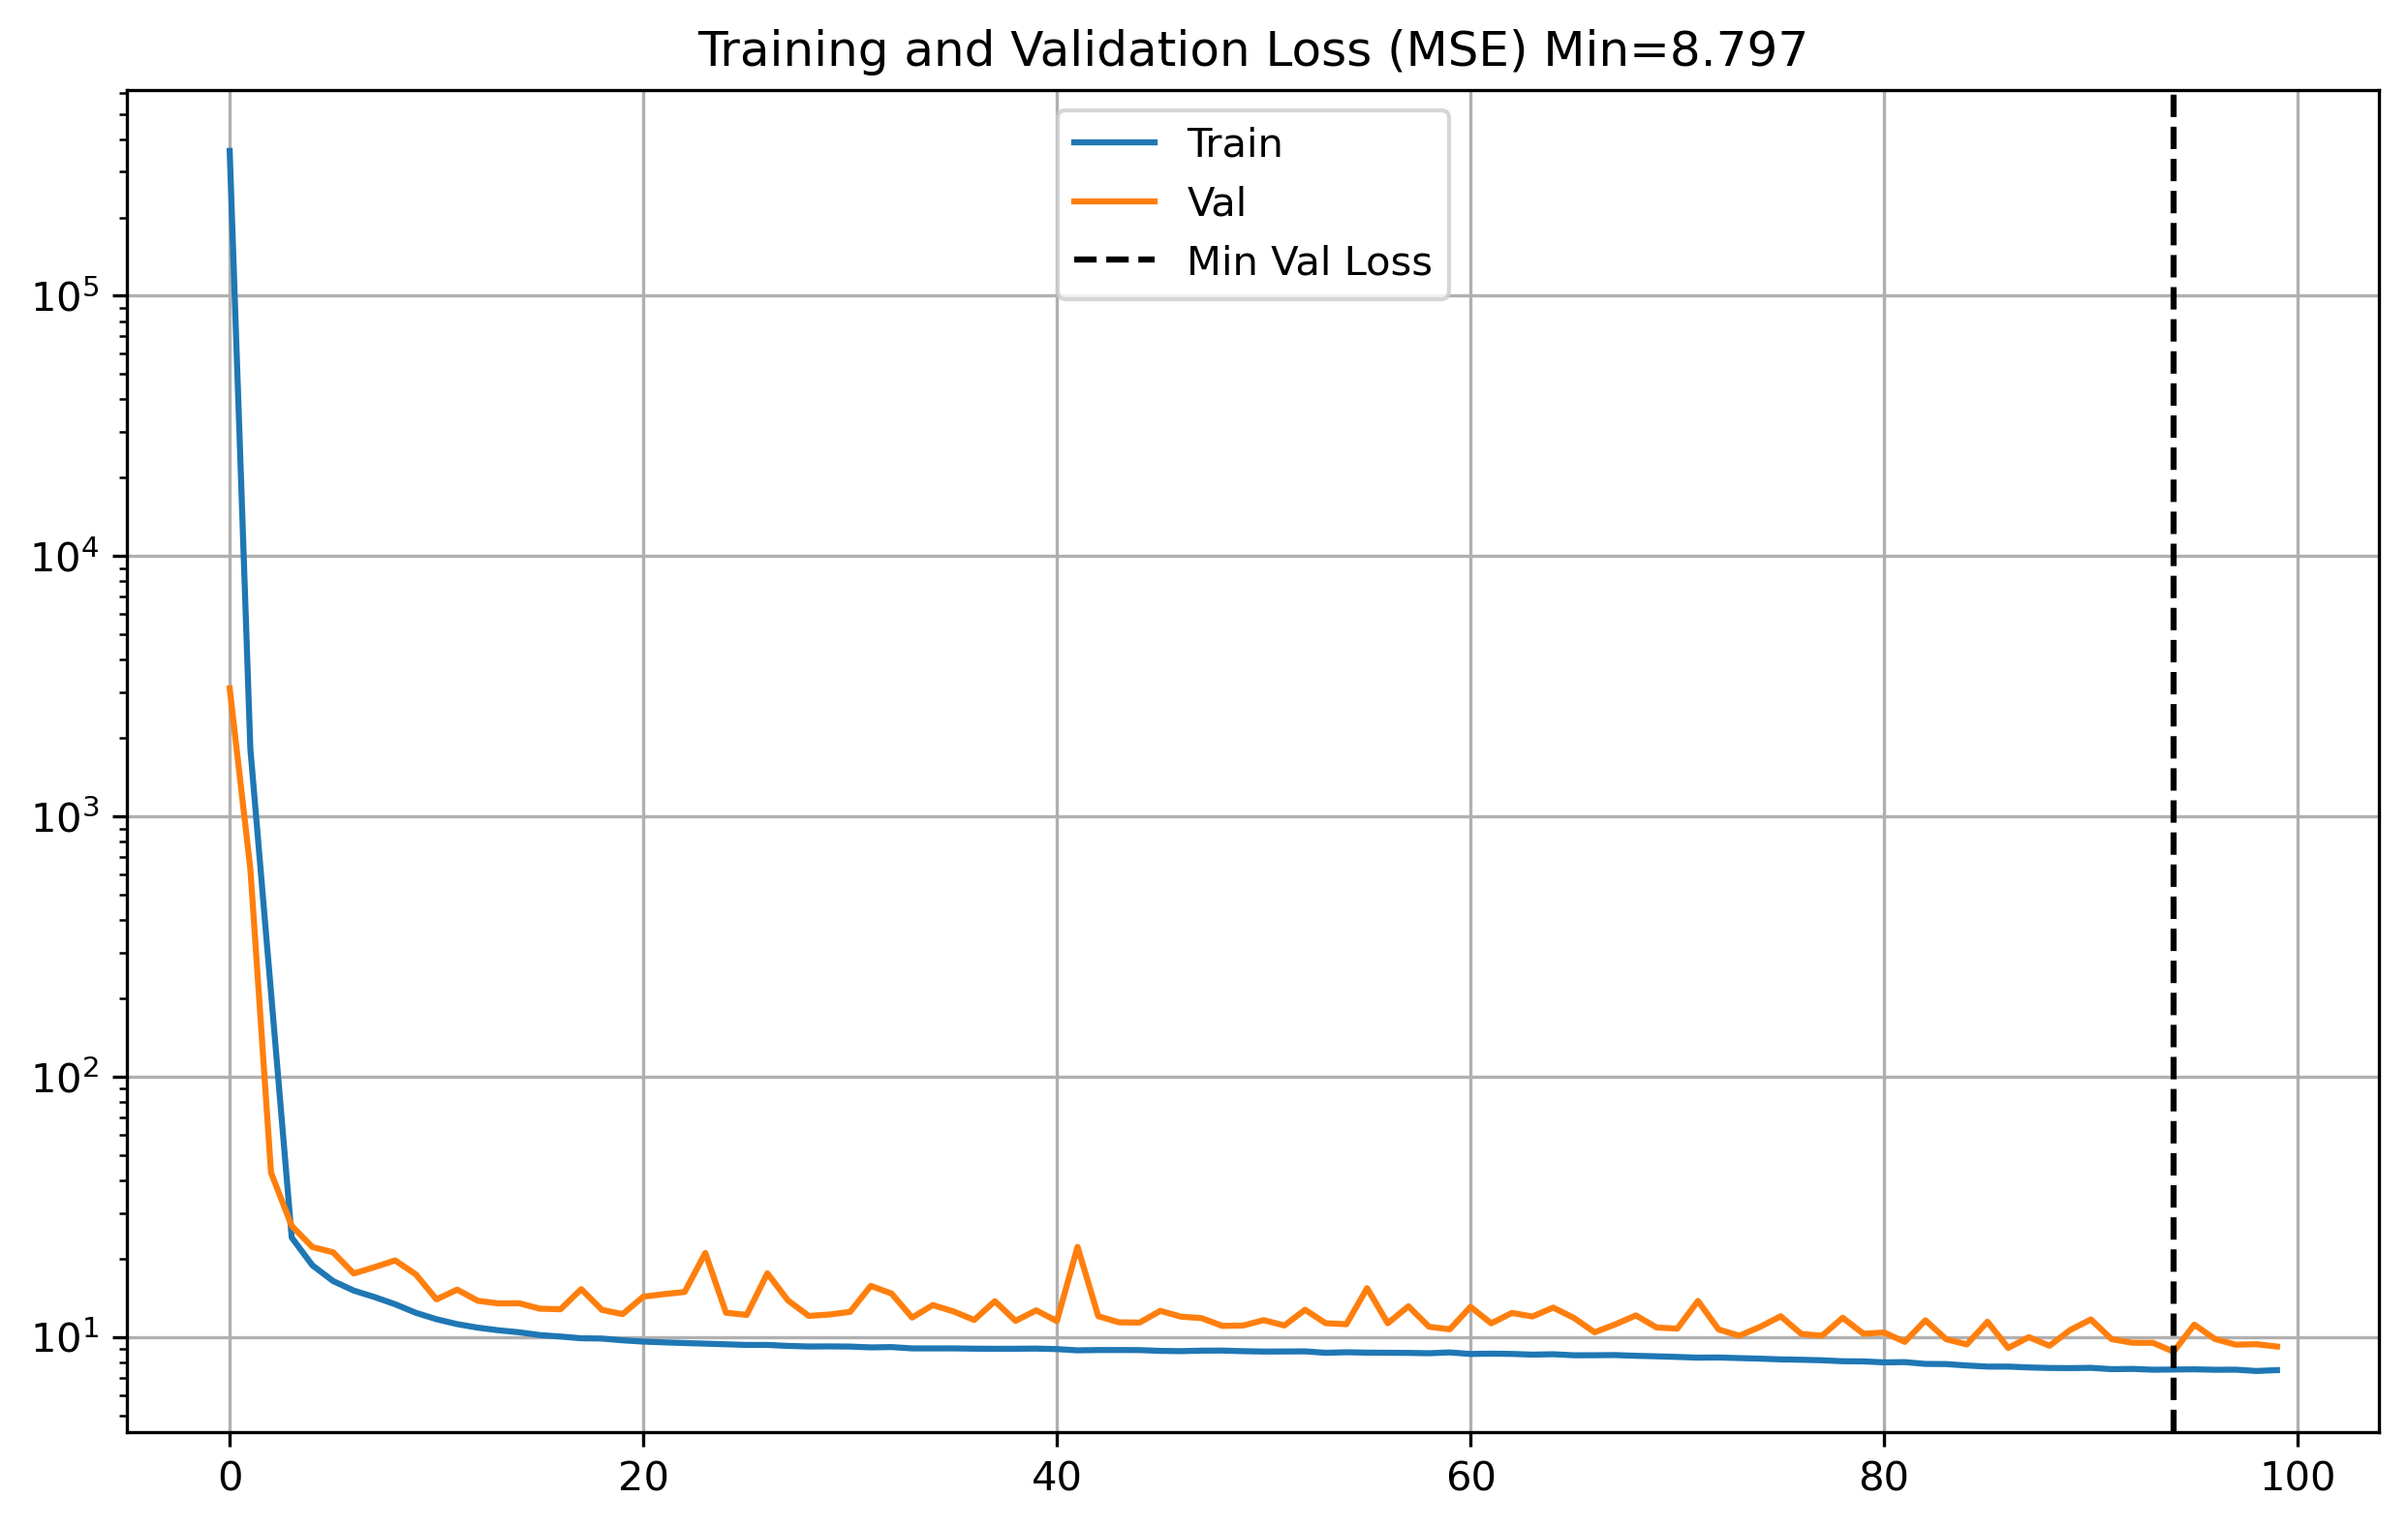
\includegraphics[scale=0.45]{train_val_loss_show.png}
                \caption{Training and Validation Loss for proposed model}
            \end{figure}
        \end{frame}

        \begin{frame}{Normalizer}{Sample Predictions}
            \begin{figure}[!htbp]
                \centering
                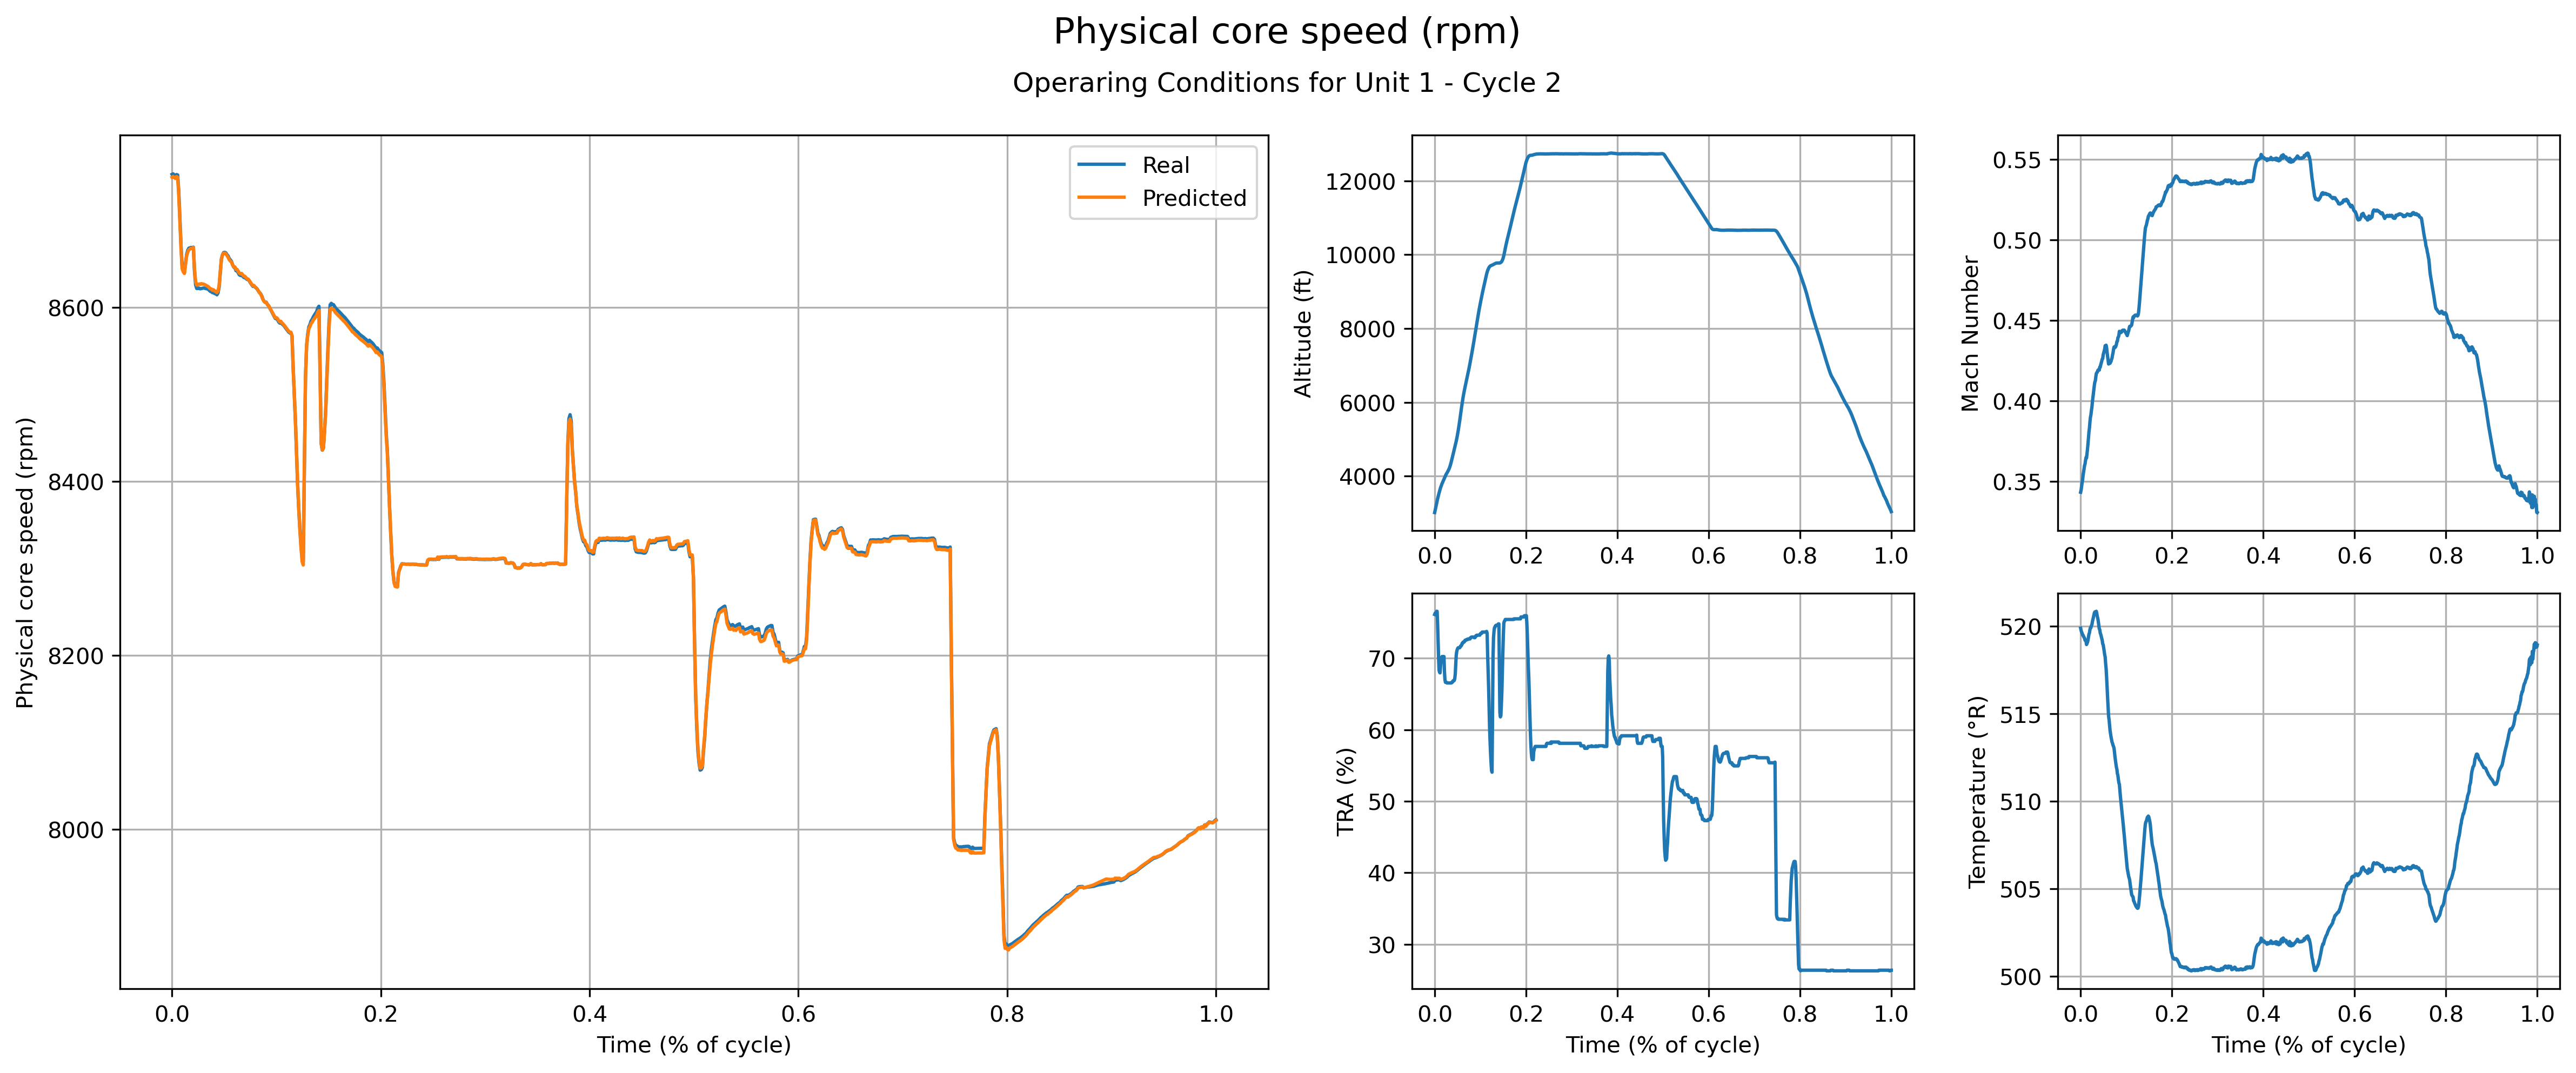
\includegraphics[scale=0.27]{Nc_cycle_2_pred_op_conditions.png}
                \caption{Comparison of Physical Core Speed predictions and real values}
            \end{figure}
        \end{frame}

        \begin{frame}{Normalizer}{Sample Predictions}
            \begin{figure}[!htbp]
                \centering
                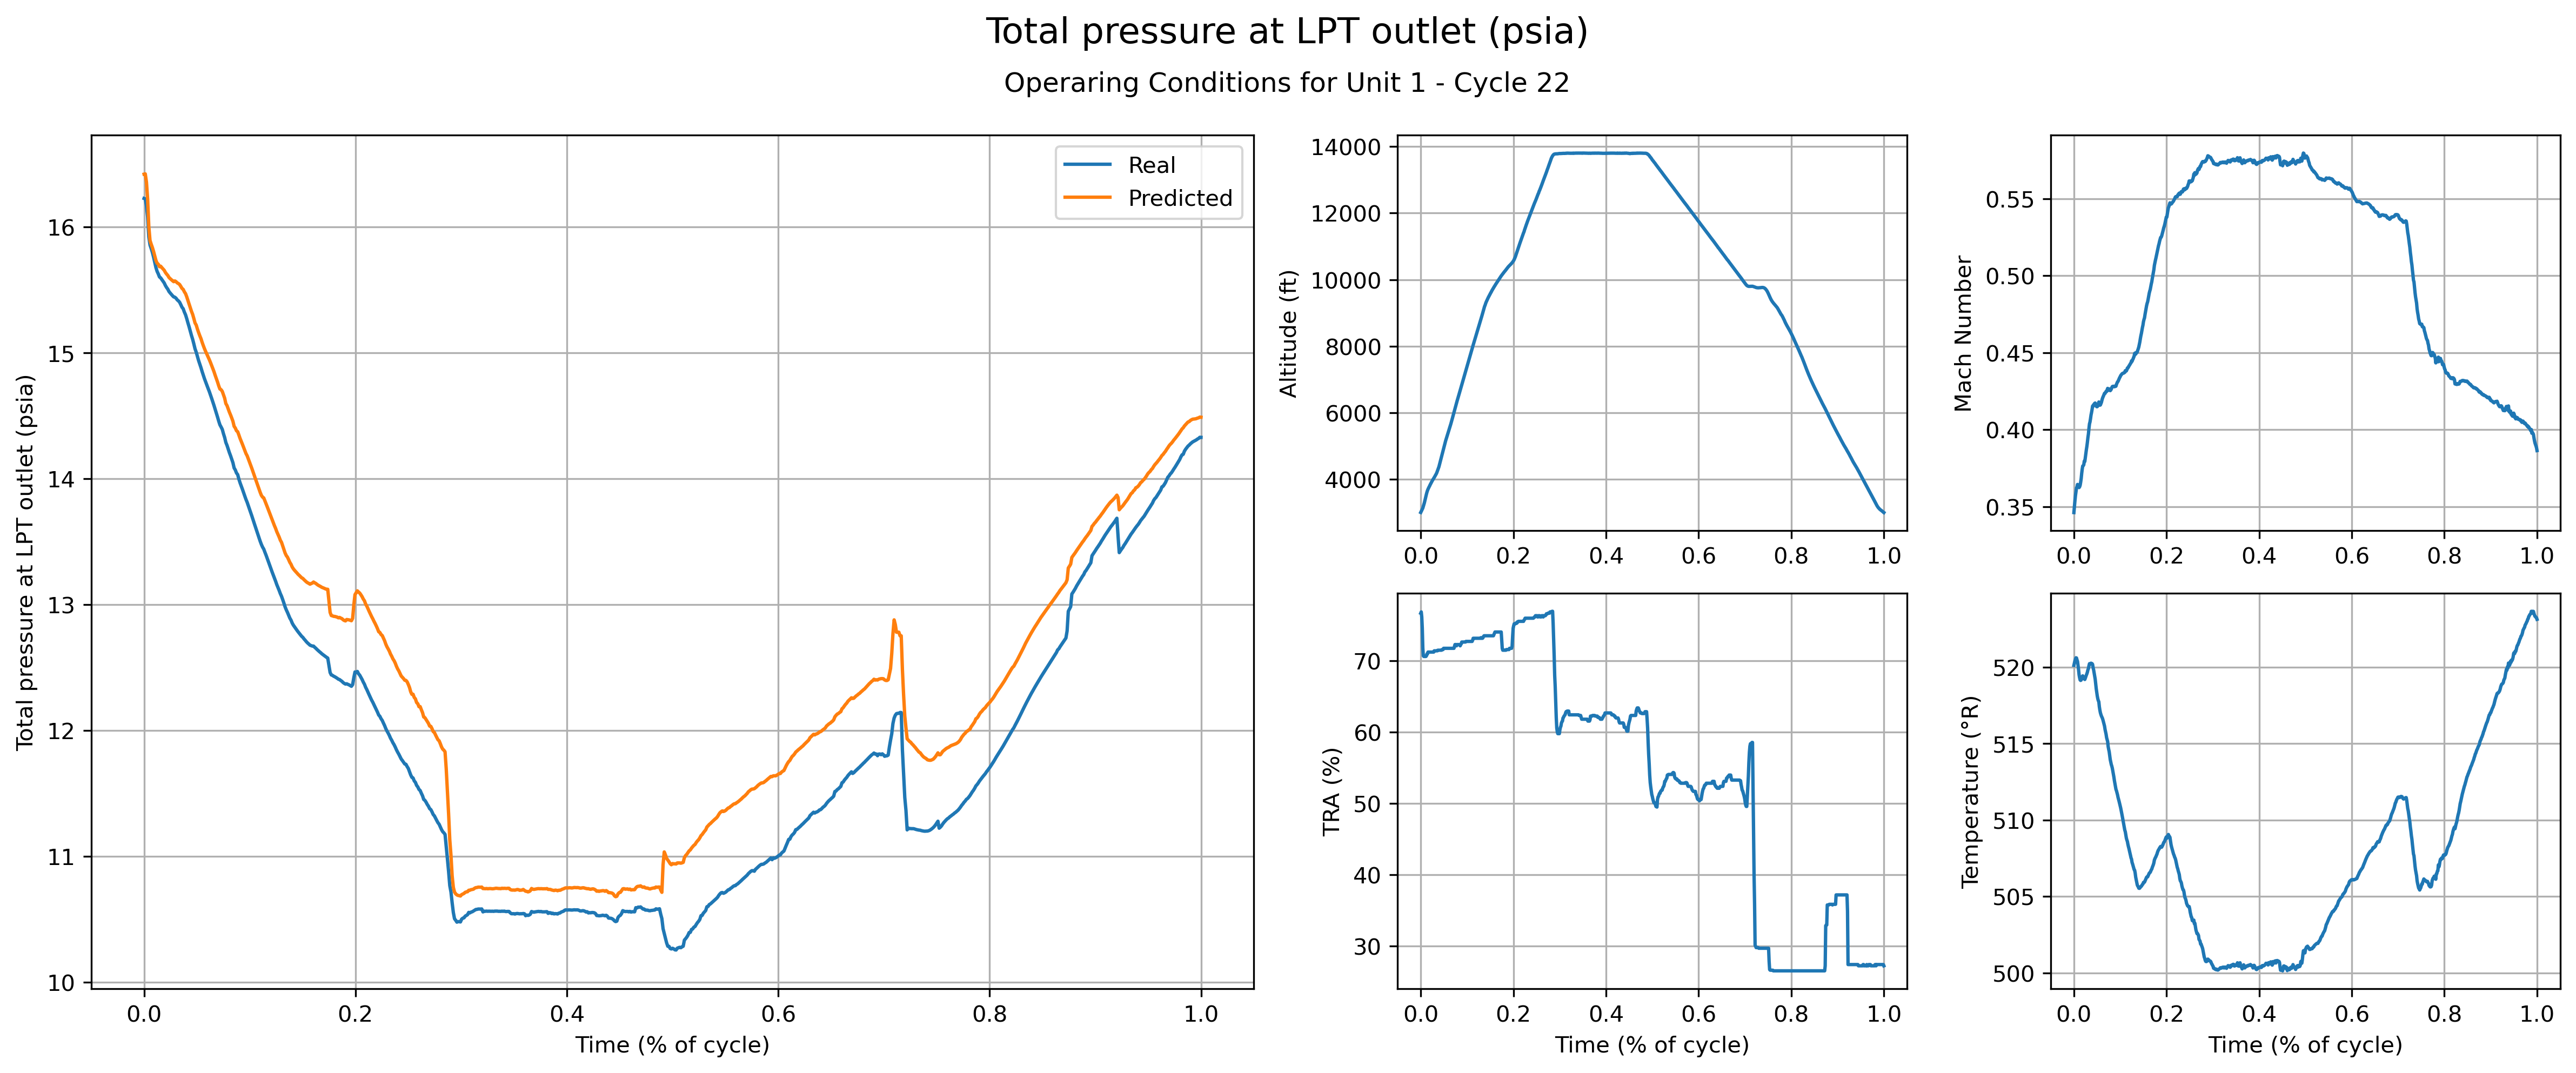
\includegraphics[scale=0.27]{P50_cycle_22_pred_op_conditions.png}
                \caption{Comparison of Total Pressure at Low Pressure Turbine outlet predictions and real values}
            \end{figure}
        \end{frame}

    \section{Conclusions}

    \section{References}
        \begin{frame}
            \frametitle{References}
            \printbibliography
    \end{frame}

\end{document}